\documentclass[uplatex,12pt]{jsarticle}
\usepackage[dvipdfmx]{graphicx}
\usepackage{url}
\usepackage{listings,jlisting}
\usepackage{ascmac}
\usepackage{amsmath,amssymb}

%ここからソースコードの表示に関する設定
\lstset{
  basicstyle={\ttfamily},
  identifierstyle={\small},
  commentstyle={\smallitshape},
  keywordstyle={\small\bfseries},
  ndkeywordstyle={\small},
  stringstyle={\small\ttfamily},
  frame={tb},
  breaklines=true,
  columns=[l]{fullflexible},
  numbers=left,
  xrightmargin=0zw,
  xleftmargin=3zw,
  numberstyle={\scriptsize},
  stepnumber=1,
  numbersep=1zw,
  lineskip=-0.5ex
}
%ここまでソースコードの表示に関する設定

\title{知能プログラミング演習II 課題5}
\author{グループ8\\
  29114003 青山周平\\
  29114060 後藤拓也\\
  29114116 増田大輝\\
  29114142 湯浅範子\\
  29119016 小中祐希\\
}
\date{2019年12月10日}

\begin{document}
\maketitle

\paragraph{提出物} group08.pdf, group08.zip
\paragraph{グループ} グループ8

\paragraph{担当}
\begin{tabular}{|c|l|}
  \hline
  氏名&担当課題\\
  \hline\hline
  青山周平&必須課題5-4, 発展課題5-7\\
  \hline
  後藤拓也&必須課題5-2, 発展課題5-6\\
  \hline
  増田大輝&必須課題5-3, 発展課題5-5\\
  \hline
  湯浅範子&必須課題5-4\\
  \hline
  小中祐希&必須課題5-1, 必須課題5-2, 発展課題5-8\\
  \hline
\end{tabular}



\section{課題の説明}
\begin{description}
\item[必須課題5-1] 目標集合を変えてみたときに,動作が正しくない場合があったかどうか,実行例を示して考察せよ.
また,もしあったならその箇所を修正し,どのように修正したか記せ.
\item[必須課題5-2] 教科書のプログラムでは,オペレータ間の競合解消戦略としてランダムなオペレータ選択を採用している.
これを,効果的な競合解消戦略に改良すべく考察し,実装せよ.
改良の結果,性能がどの程度向上したかを定量的に(つまり数字で)示すこと.
\item[必須課題5-3] 上記のプランニングのプログラムでは,ブロックの属性(たとえば色や形など)を考えていないので,色や形などの属性を扱えるようにせよ.ルールとして表現すること.
例えば色と形の両方を扱えるようにする場合,Aが青い三角形,Bが黄色の四角形,Cが緑の台形であったとする.
その時,色と形を使ってもゴールを指定できるようにする("green on blue" や"blue on box"のように)
\item[必須課題5-4] 上記5-2, 5-3で改良したプランニングシステムのGUIを実装せよ.
ブロック操作の過程をグラフィカルに可視化し,初期状態や目標状態をGUI上で変更できることが望ましい.
\item[発展課題5-5] ブロックワールド内における物理的制約条件をルールとして表現せよ.
例えば,三角錐(pyramid)の上には他のブロックを乗せられない等,その世界における物理的な制約を実現せよ.
\item[発展課題5-6] ユーザが自然言語(日本語や英語など)の命令文によってブロックを操作したり,初期状態/目標状態を変更したりできるようにせよ.
なお,命令文の動詞や語尾を1つの表現に決め打ちするのではなく,多様な表現を許容できることが望ましい.
\item[発展課題5-7] 3次元空間 (実世界) の物理的な挙動を考慮したブロックワールドにおけるプランニングを実現せよ.
なお,物理エンジン等を利用する場合,Java以外の言語のフレームワークを使って実現しても構わない.
\item[発展課題5-8] 教科書3.3節のプランニング手法を応用できそうなブロック操作以外のタスクをグループで話し合い,新たなプランニング課題を自由に設定せよ.
さらに,もし可能であれば,その自己設定課題を解くプランニングシステムを実装せよ.
\end{description}

\section{必須課題5-1}
\begin{screen}
目標集合を変えてみたときに,動作が正しくない場合があったかどうか,実行例を示して考察せよ.
また,もしあったならその箇所を修正し,どのように修正したか記せ.
\end{screen}

\subsection{手法}
用意されたサンプルプログラムにおいて、目標状態の順番を入れ替えると一例として以下のような実行結果が得られる.(中略)
\begin{lstlisting}[caption=正しくない動作例, label=mid]
***** This is a plan! *****
pick up A from the table
Place A on B
remove A from on top B
Place A on C
pick up B from the table
put B down on the table
pick up B from the table
Place B on C
pick up B from the table
Place B on C
\end{lstlisting}
​
これはプランニングがうまくいかず,中途半端な状態で終わってしまっている.\\
今回はこの現象を,目標状態を適切な順番に入れ替えるメソッドを実装することで解消した.

\subsection{実装}
以下に,今回実装したメソッドを示す.\\

\begin{lstlisting}[caption=sortGoalListメソッド, label=mid]
//目標状態を問題が起こらないように並べ替える(課題5−1)
	public ArrayList<String> sortGoalList(ArrayList<String> goalList){
		ArrayList<String> sortedGoalList = new ArrayList<String>();
		for(String s : goalList) {
			sortedGoalList.add(s);
    }
    
		for(int k = 0; k < sortedGoalList.size(); k++){
			String[] head = new String[sortedGoalList.size()];
      String[] tail = new String[sortedGoalList.size()];
      
			//各目標状態の先頭と末尾の文字を配列に格納
			for(int i = 0; i < sortedGoalList.size(); i++){
				head[i] = sortedGoalList.get(i).substring(0,1);
				tail[i] = sortedGoalList.get(i).substring(sortedGoalList.get(i).length()-1);
      }
      
			int flag = 0;
			for(int i = 0; i < sortedGoalList.size(); i++){
				for(int j = i; j < sortedGoalList.size()-i; j++){
					if(tail[i] == head[j]){
						sortedGoalList.add(j+1, sortedGoalList.get(i));
						sortedGoalList.remove(i);
						flag += 1;
						break;
					}
				}
				if(flag == 1){
					break;
				}			
			}
			if(flag == 0){
				break;
      }
      
    }
    
		return sortedGoalList;
	}
\end{lstlisting}
このメソッドの大まかな構造としては,はじめに各目標状態に含まれているアルファベット(物体名)を取得し,そのアルファベット同士を比較し適切な順番に並べ替える,というものになっている.\\
細部を順番に解説していく.まず全体の構造として,アルファベットの取得から目標状態の入れ替えまでを大きな一つの繰り返し文で囲っている.これは,目標状態の順序を入れ替えた際に目標状態のリストとアルファベットを格納している配列のインデックスが対応しなくなってしまうのを防ぐためである.\\
目標状態は一つのString型になっているため,アルファベットは先頭と末尾をsubstringsで切り取り,それぞれ別の配列に格納している.比較の部分では目標状態同士の先頭と末尾を比較し,一致したらsortedGoalList内のその二つを適切な順番に入れ替え,繰り返し文から抜け出し再び同じ処理を繰り返す.最後まで入れ替えが起こらなければflagによる判定で処理が終了する.\\
なお、このメソッドはサンプルプログラムにあるinitGoalListメソッド内で呼び出している.

\subsection{実行例}
このメソッドを用いることで以下のような目標状態であっても,正しい実行結果を得ることができる.
\begin{lstlisting}[caption=目標状態, label=mid]
goalList.add("A on B");
goalList.add("B on C");
\end{lstlisting}

\begin{lstlisting}[caption=実行結果, label=mid]
***** This is a plan! *****
pick up B from the table
Place B on A
remove B from on top A
Place B on C
pick up A from the table
Place A on B
\end{lstlisting}

\subsection{考察}
まず動作の正しくない場合についてだが,これは先述したように目標状態の順番が原因である.というのも,目標状態はリストの先頭から読み込まれるため,例のように3つの物体でプランニングを行った場合,上の二つの物体が先に積まれてしまうとその後のプランニングがうまくいかなくなるためである.\\
これの最も簡単な解消方法は,プログラム中の目標状態の記述を正しい方法に直すことであるが,これではプログラムに直接手を加える必要があるため適切ではない.\\
また,単に目標状態の順番を前後入れ替えるという方法も,汎用性が低く適切ではない.GUIから実行する場合,物体の数が3つとは限らない上,目標状態もどんな順番で入力されるかわからない.\\
よって今回は汎用性という点を考慮し,目標状態がどんな状態で入力されても順番通りに並べ替えられるような機能を実装した.\\
しかしがら,各目標状態を照合しながらの入れ替えは非常に複雑な手続きが必要であり,結果としてfor文を3重に重ねるプログラムになってしまった.物体が数個のうちは良いが,物体の数が増えるとプログラムの実行時間が爆発的に増えてしまう可能性があるので, より簡単な構造のメソッドが書けるとより良いプログラムになると考える.


\section{必須課題5-2}
\begin{screen}
教科書のプログラムでは,オペレータ間の競合解消戦略としてランダムなオペレータ選択を採用している.
これを,効果的な競合解消戦略に改良すべく考察し,実装せよ.
\end{screen}
\subsection{手法}
発展課題5-6を実装する際に利用した"ユーザーがオペレータを選択する方法"をもとに, デバックをしていき, 初期プログラムでは発生してしまう「Place A on A」や,  必須課題5-3での「Triangle on Ball」などの禁止制約をPlannigクラス, ないしはUnifierクラスを改善していった. PlannerクラスのplanningメソッドとplannnigAGoalメソッドの相互再帰構造においては, 図1をもとに簡単に説明をしたが, ここでは, その1つ1つの変数の内容まで踏み込み, UnifierクラスのMtachingメソッドまで掘り下げていく必要があった. \\

まずは, 下の図を参考に, 問題点とその改良手法を示す.
\begin{figure}[htbp]
 \begin{center}
  %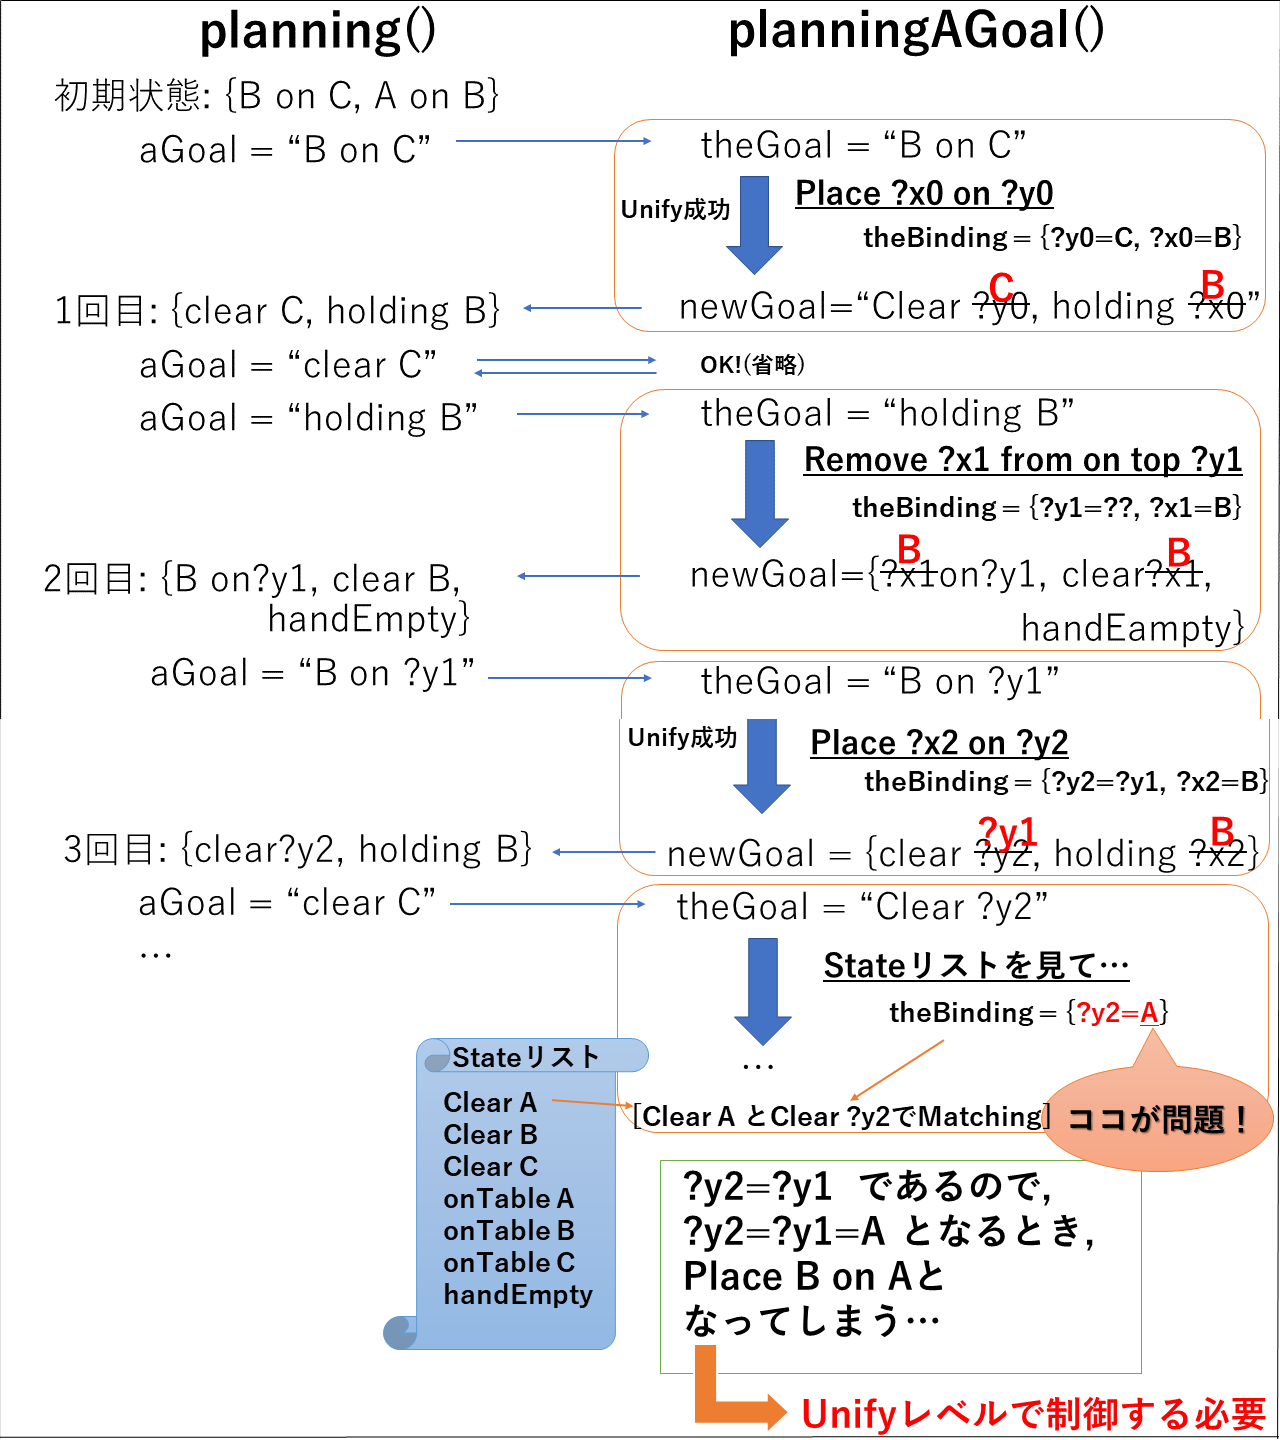
\includegraphics[width = 12cm, pagebox = cropbox, clip]{images/ishiduya.png}
 \end{center}
 \caption[]{operetarsリストの動き}\label{fig:fig1.1}
\end{figure}
上の図は, 始めの問題としては, [Aを丸, Bを台形, Cを四角]という状態で, 属性の禁止制約として[丸の上に台形や四角を置いてはいけない]が存在する中で, 「Place B on A」が成立してしまう状態を示している. planningメソッドの4つ目の内容を見てみると, y2=Aとしてバインディングされると, y2はy1ともバインディングされているため, バックトラックの結果, 「Place B on A」が成立してしまうのである. もっと具体的には, 実際にy2がバインディングされるのは, 「Clear ?y2」とStateリストを上から順にマッチングしているので, Stateリストの一番上に存在する「Clear A」とマッチングしてしまい, ?y2=Aとなるのである. ここで, 禁止制約「B on A」からマッチングが不成立(falseを返す)ようにすればよい.またこれをベースに「Place A on A」のようなバグも改良していく.\\

禁止制約もとい, 実際に生成されていく「X on Y」の関係は, 全てHashMapを使い, XをKeyとし, YをValueとして扱うことで, 物の上下関係を表現する.\\

\subsection{実装}
まずは, 属性をベースにした禁止制約をHashMapに格納していくプログラムを下に示す. これは, 課題5-3でかかわった属性クラスAttributionsで定義されている.
\begin{lstlisting}[caption=禁止制約をHashMapに管理, label=src:No1]
	//格納するHashMap
	HashMap<String,List<String>> keyValueProhibit =  new HashMap<String, List<String>>();

	// 禁止制約追加メソッド
	private void addProhibitRules() {
		System.out.println("###### Add prohibitRule ######");
		prohibitRules.add("ball on ball");
		prohibitRules.add("trapezoid on ball");
		prohibitRules.add("trapezoid on trapezoid");
		prohibitRules.add("box on ball");
		prohibitRules.add("box on box");
		prohibitRules.add("pyramid on ball");

		prohibitRules.add("ball on pyramid");
		prohibitRules.add("box on pyramid");
		prohibitRules.add("trapezoid on pyramid");
		prohibitRules.add("pyramid on pyramid");
		for(String prohibitRule: prohibitRules) {
			System.out.println("****** ProhibitRule:"+ prohibitRule+" ******");
		}
	}

	//禁止制約をHashMapのKeyとValueに格納
	public void keyValueProhibit(ArrayList<String> list){
		StringTokenizer st;
		String tokenBuffer[];
		ArrayList<String> buffer;
		ArrayList<String> xValueList = new ArrayList<String>();
		ArrayList<String> yValueList = new ArrayList<String>();
		ArrayList<String> zValueList = new ArrayList<String>();
		for(int i = 0; i < list.size(); i ++) {
			//リストの1要素をトークンに分解して
			st = new StringTokenizer(list.get(i));
			//tokenBufferに格納
			int length = st.countTokens();
			tokenBuffer = new String[length];
			for (int j = 0; j < length; j++) {
				tokenBuffer[j] = st.nextToken();
				System.out.println("tokenBuffer["+j+"] = " + tokenBuffer[j]);
			}

			//HashMapのKeyとValueを格納していく
			if(tokenBuffer[0].equals("A")) {
				xValueList.add(tokenBuffer[2]);
			}
			else if(tokenBuffer[0].equals("B")) {
				yValueList.add(tokenBuffer[2]);
			}
			else if(tokenBuffer[0].equals("C")) {
				zValueList.add(tokenBuffer[2]);
			}
		}

		keyValueProhibit.put("A", xValueList);
		keyValueProhibit.put("B", yValueList);
		keyValueProhibit.put("C", zValueList);

		System.out.println("keyValueProhibit = " + keyValueProhibit);
	}
\end{lstlisting}

addProhibitRulesで定義された禁止制約のリストを,ここでは省略しているが, 属性表現「pyramid on pyramid」から通常状態「B on A」に変換してくれるeditStatementListメソッドをかますことで, 禁止制約の表現をすべて"A, B, C"のものとして管理できる.(詳しくは, 課題5-3を参照してもらいたい). そして変換後のリストを受け取って, keyValueProhibitメソッドで「X on Y」を3つのトークンに分解し, 1つ目のトークンをKeyに, 2つ目のトークンは"on"なので無視し, 3つ目のトークンをValueに設定している.\\
禁止制約には1つのKeyに対して複数のValueを持つものが存在する(「B on A, B on B」のように...)ので, HashMapのValueはリストにしなければならなかった.\\
ここの禁止制約で, 「Place B on A」(ただし, Bは台形で, Aはボールであり, ボールの上には何も置いてはいけないという属性禁止条件が存在する)や, 「Place A on A」(根本的にあり得ない状態)などを定義することができるので, 課題5-3の内容も課題5-2の内容もまとめて処理することができる.\\

次に, 実際の推論中に生成される「X on Y」関係と, 制約条件との照らし合わせを下に示す. \\
Plannerクラスでオペレータ選択などが行われ, 実際に変数が具体化されるのは, Unifierクラスなので, その2クラスでの様子が見られる.
\begin{lstlisting}[caption=禁止制約をHashMapに管理, label=src:No1]
//Plannerクラス
 HashMap<String, String> p_productKeyOnValue; //現在の[X on Y]関係

 //AttributesクラスからPlannerクラスへ
 setHashMap(attributions.a_productKeyOnValue);

 //ゲッター
 public HashMap<String, String> getHashMap(){
	return p_productKeyOnValue;
 }
	
 //セッター
 public void setHashMap(HashMap<String, String> pHashMap){
	this.p_productKeyOnValue = pHashMap;
 }

 //planningAGoalメソッド内
 //現在のKeyOnValueリストをUnifierクラスからもらってくるため
	Unifier unification = new Unifier();
	if (unification.unify(theGoal, aState, theBinding, attributions.keyValueProhibit, p_productKeyOnValue)) {
		System.out.println("theBinding" + theBinding);

		//UnifierからもらったKeyOnValueリストを,Plannerクラスに保存
		for(String str : unification.getHashMap().keySet()) {
			System.out.println("Key = " + str + " Value = " + unification.getHashMap().get(str));
			p_productKeyOnValue.put(str, unification.getHashMap().get(str));
		}
		return 0;
	}
  }

//Unifierクラス
HashMap<String, List<String>> prohibit;	//禁止制約
HashMap<String, String> productKeyOnValue;  //現在の[X on Y]関係

 //unifyメソッド内
  //AttributionsクラスのKey制約を持ってくる
  HashMap<String, List<String>> keyProhibit = prohibit;
	if(productKeyOnValue != null) {
	   System.out.println("unify内:keyProhibit" + keyProhibit);
	}
	//これから調べる「Key on Value」の値を格納
	String[] keyOnValue = new String[2];

	for (int i = 0; i < length; i++) {
	 if (!tokenMatching(buffer1[i], buffer2[i])) {
		return false;
	 }
	 if(buffer1[1].equals("on")){
	  // 「B on C」と「?x on ?y」を考えて,
		if(i == 0){
		  keyOnValue[0] = buffer2[i];
		  System.out.println("keyOnValue[0] ="+keyOnValue[0]);
		}
		else if(i == 2){
		  keyOnValue[1] = buffer2[i];
		  System.out.println("keyOnValue[1] ="+keyOnValue[1]);
		}
	  }
	}
	//保存
	if(buffer1[1].equals("on")){
	 productKeyOnValue.put(keyOnValue[0], keyOnValue[1]);
	 System.out.println("productKeyOnValue="+productKeyOnValue);
	}

 //varMatchingメソッド内
	System.out.println("varMatchingで..." + vartoken +"と"+ token);
	System.out.println("productKeyOnValueで..." + productKeyOnValue);
	for(String str1 : productKeyOnValue.keySet()){
	 //ここは,Valueに変数「?y2」が入る
	 if(var(productKeyOnValue.get(str1))) {
	  //そのvartokenとtokenの組み合わせが,Init_KeyValueと同じだったら
	  for(String str2 : prohibit.keySet()){
	    for(int num = 0; num < prohibit.get(str2).size(); num++) {
		System.out.println("prohibit.get(str2).get("+num+") = " + prohibit.get(str2).get(num));
		if(str2.equals(str1) & prohibit.get(str2).get(num).equals(token)){
			return false;
		}
	      }
	     }
          }
	}
\end{lstlisting}
PlannerクラスとUnifierクラスで共通のリスト(produvtKeyOnValue)を共有しあい, 現在の[X on Y]の関係を保存共有する. PlannerクラスでUnifierクラスを呼び出し, その内容をトークンごとで分解し,[X on Y]の分解に基づき, KeyとValueを格納していく.
実際に, varMatchingメソッドでは, 2つ目の引数のtokenが, 次のバインディング候補であるため, それが禁止制約リストのValue値と同じであればfalseを返すようにしている.

\subsection{出力結果}
\begin{lstlisting}
unify内:keyProhibit{A=[A], B=[A, B], C=[A, C]}
varMatchingで...?y3とB
productKeyOnValueで...{B=?y3}
str2 = A
prohibit.get(str2).get(0) = A
str2 = B
prohibit.get(str2).get(0) = A
prohibit.get(str2).get(1) = B

unify内:keyProhibit{A=[A], B=[A, B], C=[A, C]}
varMatchingで...?y3とC
productKeyOnValueで...{B=?y3}
str2 = A
prohibit.get(str2).get(0) = A
str2 = B
prohibit.get(str2).get(0) = A
prohibit.get(str2).get(1) = B
str2 = C
prohibit.get(str2).get(0) = A
prohibit.get(str2).get(1) = C
Init_Key(str) = A
Init_Key(str) = B
Init_Key(str) = C
theBinding{?y0=C, ?x0=B, ?y2=C, ?x2=B, ?y3=C, ?x3=B}
\end{lstlisting}
上は出力結果の一部を示している. Attributesクラスでの禁止制約がPlannerクラスそして, Unifierクラスにうまく用いられ, keyProhibitとして出力されていることが分かる.\\
はじめは {?y3とB}でマッチングを行うところであり, それが「X on Y」関係を持つように, HashMapのproductKeyOnValueに保存されている. そして, 「B on ?y3」に当てはまるものを禁止制約と照らし合わせている. 「B on A」や「B on B」が実行されようとしているので,禁止制約が発動していることがわかる. 次に「B on ?y3」に当てはまる候補として, Cが用いられ, 「B on C」は大丈夫であるので, {?y3=C}と具体化されている.

\subsection{考察}
PlannerクラスとUnifierクラスで共通のリストがあるおかげで, 離れたバインディ状態(?y3=?y2があり, その後?y3=Cとなる状態)でもしっかりと具体化することができてた. 上手く禁止制約条件をUnifyのMatchingメソッドまで行えたが, 「Aを取ってBの上に置く」と「AをBから取り除く」などのループ処理が行われているため, プランニングが無限に陥る可能性が取り除けていない. 制約条件ではじいたあとの処理をさらに考える必要があった.

\subsection{感想}
出力結果とプログラムを理解していくのがとても大変であった. 初期プログラムの出力だけでは, なにが起こっているのか全く分からない. 分岐箇所やメソッドに結果などを細かく出力していくことで, プログラムを解読できた.\\
また, PlannerクラスはPlanningメソッドとPlanningAGoalメソッドの再帰構造によるバックトラックだったので, プログラムの改良がとても難しかった. 「Place A on B」を一つとっても, いろいろな処理をしたのちに, 最終的にこの結果が出てくるのであって, その内部構造の理解が必須だった. まだ, 改良点や, 不具合が多いので, これからの課題でさらに深めていきたい.


\section{必須課題5-3}
\begin{screen}
    上記のプランニングのプログラムでは,ブロックの属性(たとえば色や形など)を考えていないので,色や形などの属性を扱えるようにせよ.ルールとして表現すること.
    例えば色と形の両方を扱えるようにする場合,Aが青い三角形,Bが黄色の四角形,Cが緑の台形であったとする.
    その時,色と形を使ってもゴールを指定できるようにする("green on blue" や"blue on box"のように)
\end{screen}
\subsection{手法}
ブロックの属性を扱えるようにするために,まずはルールによってブロックと属性の関係を表現し,それらの関係を保持する必要がある.
その上で,属性によって表現されたゴールや,初期状態をブロックによる表現に変換し,後ろ向き推論を行う方針とした. \\
ここで,ブロックの属性によってゴールを表現する場合,そのまま後ろ向き推論を行うと,同一ブロックの異なる属性による表現がワーキングスペースに含まれる場合などへの対応が非常に複雑となる.
したがって,入力されたルールと初期状態はあらかじめ属性表現をブロックに変換することで,もとの後ろ向き推論が正常に機能するような実装を行うものとする.

\subsection{実装}
まず,属性を扱うクラスAttributionsを作成した.
Attributionsクラスの変数としてHashMap<String,String>型のattributions,List<String>型のrulesがある.
それぞれ,属性とブロックの関係(属性が主キー)の集合,ルールの集合に対応する.
このAttributionsクラスには以下の3つのコンストラクタが存在し,全て上記変数への操作を行うものであるが,それぞれに次のような用途がある.

\begin{description}
    \item[Attributions()] テスト用のデフォルトコンストラクタ.デフォルトのルールが用意されている.ルールは自然言語で記述.
    \item[Attributions(List \textless String\textgreater rules)] 自然言語で記述されたルールをもとに属性とブロックの関係を構築する.
    \item[Attributions(HashMap \textless String, String\textgreater attributions)] あらかじめ,属性とブロックの関係が構築された状態のものを受け取る.
\end{description}
ただし,自然言語で記述されているものは,"ブロック is 属性"の形で表現されているものを扱うものとする.
例えば,"A is blue"と記述されたものを受理する. \\

次に,自然言語から属性とブロックの関係を構築するメソッドaddAttribution(String attributionState)についての説明を行う.
このメソッドは上記コンストラクタAttributions()とAttributions(List \textless String\textgreater rules)から呼び出される.
これらのコンストラクタからはrulesの各要素を引数として渡すものとする.
addAttributionメソッドは仮引数attributionStateでこれらを受け取り,"ブロック is 属性"を空白で分割したリストの第二要素が"is"である場合に,attributionsに関係を加える.
この時,属性を主キーとし,ブロックを紐づけられるオブジェクトとする. \\
すなわち,"A is blue"とした場合には,第二要素は"is"であるので"blue"を主キーとして,"A"と紐づけられることとなる. \\

以上により,属性を持つブロックを扱うための下準備が整った. \\

続いて,attributionsに格納された属性とブロックの関係をゴールリストや初期状態のリストに適応するためのメソッドeditStatementList(ArrayList<String> statementList)についての説明である.
このメソッドでは,仮引数として渡されたstatementListの各要素について,attributions内に格納されている属性との照合作業が行われ,属性がある場合には紐づけられたブロック名に置き換えられる作業が行われる.
以下にメソッドのソースコードを示す.
\begin{lstlisting}[caption=editStatementListメソッドの実装, label=mid]
    ArrayList<String> editStatementList(ArrayList<String> statementList) {
		System.out.println("++++++ EditStatement ++++++");
		ArrayList<String> newStatementList = new ArrayList();
		for (String statement: statementList) {
			List<String> tokens = Arrays.asList(statement.split(" "));
			String newStatement = "";
			for(int tokenNum = 0; tokenNum < tokens.size(); tokenNum++) {
				String token = tokens.get(tokenNum);
				if(attributions.containsKey(token)) {
					token = attributions.get(token);
				}
				newStatement += token;
				if(tokenNum < tokens.size()-1) {
					newStatement += " ";
				}
			}
			newStatementList.add(newStatement);
			System.out.println(statement+" =====> "+newStatement);
		}
		return newStatementList;
	}
\end{lstlisting}
特に,9~11行目でHashMapの機能を利用して属性からブロック名を導き出す処理を行っている.

以上によって,自然言語で記述されたルール集合から導出された属性とブロックの関係や与えられた属性とブロックの関係を元にして,
ゴールリストや初期状態のリストに含まれる属性表現をブロック名に統一する処理が完成した.

具体的な利用法は,使用したい任意のコンストラクタによってAttributionsクラスを初期化し,以下のような形で,ゴールリストや初期状態のリストに適用すればよい.
\begin{lstlisting}[caption=editStatementListの利用, label=mid]
    goalList = attributions.editStatementList(initAttributeGoalList());
	initialState = attributions.editStatementList(initAttributeInitialState());
\end{lstlisting}


\subsection{実行例}
以下に,CUI上での実行結果を示す.
ただし,コンストラクタはデフォルトコンストラクタを使用するものとする.
\begin{lstlisting}[caption=ゴールと初期状態に属性を指定した場合の実行結果, label=mid]
    ~/Programming2/Work5
    ●java Planner                                                                                                                                                                                                     【 re-fix/attribute-rule 】
    ========== goal:green on ball ==========
    ========== goal:blue on pyramid ==========
    ++++++ EditStatement ++++++
    green on ball =====> B on C
    blue on pyramid =====> A on B
    ---------- initInitialState:clear blue ----------
    ---------- initInitialState:clear green ----------
    ---------- initInitialState:clear red ----------
    ---------- initInitialState:ontable box ----------
    ---------- initInitialState:ontable pyramid ----------
    ---------- initInitialState:ontable ball ----------
    ---------- initInitialState:handEmpty ----------
    ++++++ EditStatement ++++++
    clear blue =====> clear A
    clear green =====> clear B
    clear red =====> clear C
    ontable box =====> ontable A
    ontable pyramid =====> ontable B
    ontable ball =====> ontable C
    handEmpty =====> handEmpty
    *** GOALS ***[B on C, A on B]
    **B on C
    Place B on C
    *** GOALS ***[clear C, holding B]
    **clear C
    [clear A, clear B, clear C, ontable A, ontable B, ontable C, handEmpty]
    *** GOALS ***[holding B]
    **holding B
    pick up B from the table
    *** GOALS ***[ontable B, clear B, handEmpty]
    **ontable B
    [clear A, clear B, clear C, ontable A, ontable B, ontable C, handEmpty]
    *** GOALS ***[clear B, handEmpty]
    **clear B
    [clear A, clear B, clear C, ontable A, ontable B, ontable C, handEmpty]
    *** GOALS ***[handEmpty]
    **handEmpty
    pick up B from the table
    Place B on C
    [clear A, ontable A, ontable C, B on C, clear B, handEmpty]
    *** GOALS ***[A on B]
    **A on B
    Place A on B
    *** GOALS ***[clear B, holding A]
    **clear B
    [clear A, ontable A, ontable C, B on C, clear B, handEmpty]
    *** GOALS ***[holding A]
    **holding A
    pick up A from the table
    *** GOALS ***[ontable A, clear A, handEmpty]
    **ontable A
    [clear A, ontable A, ontable C, B on C, clear B, handEmpty]
    *** GOALS ***[clear A, handEmpty]
    **clear A
    [clear A, ontable A, ontable C, B on C, clear B, handEmpty]
    *** GOALS ***[handEmpty]
    **handEmpty
    pick up A from the table
    Place A on B
    ***** This is a plan! *****
    pick up B from the table
    Place B on C
    pick up A from the table
    Place A on B
\end{lstlisting}
まず,3・4行目で属性によってゴールが表現されていること示している.
その次に,5~7行目でこれらのゴールを属性からブロック名による表現に変換している.
続いて,8~14行目で属性によって式状態が表現されていることを示している.
先ほどと同様に,15~22行目では,これらの表現を属性によるものからブロック名のみの形に変更している.
したがって,以降の実行結果はブロック名のみを用いた場合と同様となる.

\subsection{考察}
属性を扱うに当たって,初めは属性のまま推論を行い,プランニングを実行できるようにしようと考えた.
しかし,同じブロックの属性であっても,異なる属性同士において,字面だけではマッチングが成功しないことに気が付いた.
例えば"A is blue"と"A is box"がルールとして与えられていたとする.
この時,ゴールが"blue on green"で,状態として"box on green"が保持されているものとする.
本来,blueとboxは同じブロックAの属性であるが,字面の上では,異なる定数として認識される. \\
これらを同一のブロックAを指し示すものとして認識するには,属性からブロックそのものへと変換する機能が必要である.
したがって,変換後のゴール"A on B"と状態"A on B"であればマッチングは成功する. \\
ここで,もう一度属性のまま推論を行う意義を考えることとした.
上記の方法では,マッチングにおいて最終的に属性からブロック名への変換処理を行っている.
ところが,初めから同様に属性をブロック名に変換する手法にすることでもマッチングは可能である.
例えば,あらかじめゴールを"blue on green"から"A on B"に変換し,初期状態を全てブロック名による表現にすることで,プランニング中の状態を"A on B"とする.
結果として,即座に"A on B"と"A on B"のマッチングが行われるようにする. \\
加えて,後者の方がゴールリストと初期状態のリストから属性表現をブロック名に変換するのみであるので,処理も非常にシンプルとなる.
後ろ向き推論の特徴と処理の簡潔さから,後者の手法を採用することにした. \\
複数ある実現方法の中から,既存のプログラムとの相性や論理的な汎用性を考えてもっとも良いと思える方法を選択できたと考えている.


\section{必須課題5-4}
\begin{screen}
    上記5-2, 5-3で改良したプランニングシステムのGUIを実装せよ.\par
    ブロック操作の過程をグラフィカルに可視化し,初期状態や目標状態をGUI上で変更できることが望ましい.
\end{screen}
湯浅の担当箇所は,得られた結果を基にしたGUI本体の実装である. \\
青山の担当箇所は,必須課題5-4におけるGUIとPlanner.javaとの間でデータの仲介を行うPresenterの制作である.

\subsection{手法}
\noindent (湯浅担当) \\
GUIで求められる出力が行えるように,以下のような機能を加えた.

\begin{itemize}
\item ブロック操作の過程を示す
\item ブロック操作の過程をグラフィカルに可視化する
\item 初期状態と目標状態をGUI上から画面入力で変更できる
\item 属性の決定をGUI上から行える
\item 操作に必要なオペレータと属性のデータを表示する
\item 禁止制約によってブロック操作が停止した場合にそれを表示する
\end{itemize}

これらのプログラムを実装するためのデータ受け渡し部分は青山君が作成してくれるため,ここでは受け取ったデータを基にしてどのような方法で表示を行うか考えながら実装を行った.実装はSwingによって行った.\\

また今回は初めてのGUI作成であったため,第一週では受け取るデータを既に取得したと仮定し,自ら作成した仮データを基にしてGUIについての検討を行った.第二週では実際にデータを受け取り,そのデータを基に正しく描画やプランニングが行えるようにプログラムを改良した.\\

\noindent (青山担当) \\
Presenterを実装するにあたり,以下のような方針を立てた.
\begin{enumerate}
\item Planner.javaのデータを,外部から取り出し,セットできるように改良する.
\item 導かれたプランの導出過程を渡せるようにする.
\end{enumerate}

1.に関して,MVPアーキテクチャを導入し,GUIとPlanner間のデータのやり取りを,Presenterによって緩衝することで,拡張性の向上とGUI担当者の負担軽減を図った.

2.に関して,GUI担当者が受け取りやすい渡し方を相談して決めることで,柔軟に対応した.

\subsection{実装}
\noindent (湯浅担当) \\
作成したGUIプログラムの中の主部分についての実装を以下に示す.\\

まず,GUIプログラムのmeinメソッドをソースコード\ref{main}に示す.
\begin{lstlisting}[caption=mainメソッド,label=main]
public static void main(String[] args){
	// 画像の定義
	images = new String[5][4];
	images[0][0] = "image/squBt.png";
	・・・
	images[4][3] = "image/daiDeft.png";

	// 対応番号の指定(色・形それぞれで定義)
	imageMapC = new HashMap<>();
	imageMapC.put("Blue", 0);
	・・・
	imageMapC.put("Default", 4);
	imageMapS = new HashMap<>();
	・・・

	// 属性指定での入出力に対応(defaultは予め弾く)
	Attribution = new HashMap<>();
	Attribution.put("Blue", 1);
	・・・
	Attribution.put("Yellow", 1);
	Attribution.put("box", 2);
	・・・
	Attribution.put("trapezoid", 2);

	PGUI frame = new PGUI();
	frame.setDefaultCloseOperation(JFrame.EXIT_ON_CLOSE);
	frame.setBounds(10, 10, 650, 450);
	frame.setTitle("プランニングシステム");
	frame.setVisible(true);
}
\end{lstlisting}
ここでフレームの大きさと表示位置・タイトルや,フレームを閉じると同時にプログラムを終了させるなどの動作を定めた.さらに,プログラム中で使用する変数であらかじめ値を設定しておくものの定義を行った.\\

次に,GUIプログラムのコンストラクタをソースコード\ref{PGUI}に示す.
\begin{lstlisting}[caption=コンストラクタ,label=PGUI]
PGUI(){
	// プレゼンターとの連結
	presenter = new Presenter();
	// 結果の格納(メソッド呼び出し)
	ArrayList<String> result = presenter.getPlan();
	results = new ArrayList<>(result);
	// 初期状態の追加
	results.add(0, "default position");
	// 結果ステップデータの取得
	pUR = presenter.getStepList();
	// 入力デフォルト値の格納(メソッド呼び出し)
	initialState = presenter.getInitialState();
	// 出力デフォルト値の格納(メソッド呼び出し)
	goalList = presenter.getGoalList();
	// 初期状態の格納
	String[] initialName = {"A", "B", "C"};
	String[] initialAColor = {"Default", "Default", "Default"};
	String[] initialAShape = {"default", "default", "default"};
	for (int i = 0; i < initialName.length; i++) {
		modelName.addElement(new String(initialName[i]));
		modelColor.addElement(new String(initialAColor[i]));
		modelShape.addElement(new String(initialAShape[i]));
	}
	// 禁止制約の格納
	prohibitRules.add("box on pyramid");
	・・・
	prohibitRules.add("trapezoid on ball");

	// 2ページ目以降のカード作成用メソッド
	createResultPage(pUR);
	// ボタンの作成メソッド
	createButton();
	// 最終処理メソッド
	finishData();
}
\end{lstlisting}
PGUIコンストラクタでPresenterプログラムを起動し,プランニングを行った結果を取得する.また同時に初期状態をGUIで表示するため,これらの情報も格納した.\\

ここから,先に述べた各機能の実装について詳しく記述していく.\\
まず始めにブロック操作の過程を示すプログラムをソースコード\ref{katei}に示す.
\begin{lstlisting}[caption=過程表示,label=katei]
JPanel tostring2 = new JPanel();
tostring2.setLayout(new BoxLayout(tostring2, BoxLayout.PAGE_AXIS));
tostring2.setBackground(Color.WHITE);
ArrayList<String> printResult = presenter.getPlan();
tostring2.add(new JLabel("***** This is a plan! *****"));
for (String printR : printResult) {
	tostring2.add(new JLabel(printR));
}
JScrollPane scrollpane2 = new JScrollPane(tostring2);
scrollpane2.setPreferredSize(new Dimension(200, 310));
BevelBorder border2 = new BevelBorder(BevelBorder.LOWERED);
scrollpane2.setBorder(border2);
JPanel Plan = new JPanel();
Plan.setLayout(new BoxLayout(Plan, BoxLayout.PAGE_AXIS));
Plan.add(new JLabel("Plan "));
Plan.add(scrollpane2);
\end{lstlisting}
ブロック操作の過程を示すため,新しく作成したパネルに受け取ったリストデータをラベルとして加え,そのパネルをフレームに追加することで表示を行った.また経路が長くなったときを考え,必要に応じてスクロールバーを追加できるようにした.\\

次にブロック操作の過程をグラフィカルに可視化するためのプログラムをソースコード\ref{graphic1},\ref{graphic2}に示す.このとき初期状態は別で取得するため,初期状態のみを描画するプログラムと,以降の過程を描画するプログラムを分けて作成した.
\begin{lstlisting}[caption=グラフィカル表示1(一部抜粋),label=graphic1]
// 変数決定,属性名の初期化,配置用・アーム用座標配列を定義
・・・
// 2ページ目の設定
JPanel page2 = new JPanel();
JLabel[][] p2Label = new JLabel[row][col];
GridLayout page2layout = new GridLayout();
page2layout.setRows(row); // 行数
page2layout.setColumns(col); // 列数
page2.setLayout(page2layout);
// テーブルの上に乗っているブロックの初期化
int next = 0;
for (String dataS : dataTable) {
	String[] state = dataS.split(" ", 0);
	for (int i = 0; i < blocks.size(); i++) {
		// 初めに入手したブロック名が何番目のものかcheck
		if (state[1].equals(blocks.get(i))) {
			// 名称一致のとき
			iconX[i] = row - 1;
			iconY[i] = next;
			next++;
		}
	}
}
// 他ブロックの上に乗っているブロックの初期化
for (String dataS : dataOn) {
	String[] state = dataS.split(" ", 0);
	for (int i = 0; i < blocks.size(); i++) {
		// それぞれの属性の番号を取得
		if (state[0].equals(blocks.get(i))) {
			ue = i;
		} else if (state[2].equals(blocks.get(i))) {
			sita = i;
		}
	}
	// 上部分の座標の確定
	iconX[ue] = iconX[sita] - 1;
	iconY[ue] = iconY[sita];
}
// blockとアームの上書き
for (int i = 0; i < blocks.size(); i++) {
	p2Label[iconX[i]][iconY[i]] = new JLabel(icon[i]);
	p2Label[iconX[i]][iconY[i]].setText(iconName[i]);
}
p2Label[armX][armY] = new JLabel(arm);
p2Label[armX][armY].setText(armname);
// アイコンの挿入
for (int i = 0; i < row; i++) {
	for (int j = 0; j < col; j++) {
		page2.add(p2Label[i][j]);
	}
}
\end{lstlisting}


\begin{lstlisting}[caption=グラフィカル表示2(一部抜粋),label=graphic2]
// 3ページ目以降
for (int i = 0; i < cardPage; i++) {
	// 初期化(2ページ目作成と同様の操作)
	・・・
	String hatenaX = pUR.get(i).getBindings().get("?x");
	String hatenaY = pUR.get(i).getBindings().get("?y");
	int hXz = blocks.indexOf(hatenaX);
	int hYz = blocks.indexOf(hatenaY);
	if (pUR.get(i).getName().equals("Place ?x on ?y")) {
		// xの操作
		iconX[hXz] = iconX[hYz] - 1;
		iconY[hXz] = iconY[hYz];
		// アームの操作
		armX = iconX[hXz] - 1;
		armY = iconY[hYz];
	} else if (pUR.get(i).getName().equals("remove ?x from on top ?y")) {
		// xの操作
		iconX[hXz] = iconX[hXz] - 1;
		iconY[hXz] = iconY[hYz];
		// アームの操作
		armX = iconX[hXz] - 1;
		armY = iconY[hYz];
	} else if (pUR.get(i).getName().equals("pick up ?x from the table")) {
		// xの操作
		iconX[hXz] = iconX[hXz] - 1;
		iconY[hXz] = iconY[hXz];
		// アームの操作
		armX = iconX[hXz] - 1;
		armY = iconY[hXz];
	} else if (pUR.get(i).getName().equals("put ?x down on the table")) {
		// xの操作,アームの操作
		iconX[hXz] = row - 1;
		armX = iconX[hXz] - 1;
		boolean umu;
		for (int j = 0; j < col; j++) {
			umu = true;
			for (int k = 0; k < iconY.length; k++) {
				if (j == iconY[k]) {
					umu = false;
					break;
				}
			}
			if (umu == true) {
				iconY[hXz] = j;
				armY = j;
				break;
			}
		}
	}
	// block・アームの上書き,アイコンの挿入
	・・・
}
\end{lstlisting}
上のように,初期状態は別のメソッドから受け取り予め描画を行い,そのデータを基にしてブロック操作の過程を描画した.また描画は座標で管理を行った.\\

さらに,初期状態と目標状態・各ブロックの属性をGUI上から変更,表示するためのプログラムをソースコード\ref{TextArea}と\ref{JList}に示す.
\begin{lstlisting}[caption=初期状態と目標状態の変更,label=TextArea]
// 手動入力用パネル
JPanel natural = new JPanel();
natural.setLayout(new BoxLayout(natural, BoxLayout.PAGE_AXIS));
// 入力(setInitialState)
JPanel sI = new JPanel();
iArea = new JTextArea(9, 20);
JScrollPane iScroll = new JScrollPane(iArea);
String ii = "";
for(String i : initialState) {
	ii += i + "\n";
}
iArea.setText(ii);
sI.add(iScroll);
// 入力(setGoal)
JPanel sG = new JPanel();
gArea = new JTextArea(4, 20);
JScrollPane gScroll = new JScrollPane(gArea);
String gg = "";
for(String g : goalList) {
	gg += g + "\n";
}
gArea.setText(gg);
sG.add(gScroll);
natural.add(sI);
natural.add(sG);
\end{lstlisting}
JTextAreaを用いて文字列の入力がGUI上で行えるようにした.また,入力文が増えた場合のためスクロールバーを必要に応じて表示した.\\

\begin{lstlisting}[caption=各ブロックの属性変更,label=JList]
JPanel allRadio = new JPanel();
// 色選択
JPanel p2 = new JPanel();
radio = new JRadioButton[4];
radio[0] = new JRadioButton("Blue");
・・・
// ボタンのグループ化
ButtonGroup group = new ButtonGroup();
group.add(radio[0]);
・・・
p2.add(new JLabel("Select Color"));
p2.add(radio[0]);
・・・
// 形状選択(色選択と同様の操作)
・・・

// 属性編集用ボタンの作成
JPanel ADS = new JPanel();
ADS.add(new JLabel("new Name "));
newNameText = new JTextField(5);
ADS.add(newNameText);
JButton add = new JButton("追加");
add.addActionListener(this);
add.setActionCommand("addButton");
ADS.add(add);
・・・
allRadio.add(ADS);
allRadio.add(p2);

// 属性入力用パネルの作成
JPanel attribution = new JPanel();
JPanel p4 = new JPanel();
// 属性の決定用パネル
JPanel nameD = new JPanel();
nameD.add(new JLabel("Determine Attribution "));
p4.add(nameD);
JPanel attribute = new JPanel();
JPanel NAME = new JPanel();
・・・
// リストで実現
namelist = new JList(modelName);
JScrollPane namesp = new JScrollPane();
namesp.getViewport().setView(namelist);
NAME.add(namesp);
attribute.add(NAME);
// 色選択リストパネル
colorlist = new JList(modelColor);
JScrollPane colorsp = new JScrollPane();
colorsp.getViewport().setView(colorlist);
// リストを選択不可にする
colorlist.setEnabled(false);
colorsp.setBorder(borderC);
JPanel COLOR = new JPanel();
・・・
COLOR.add(colorsp);
attribute.add(COLOR);
// 形状選択リストパネル(色選択と同様の操作)
・・・
p4.add(attribute);
\end{lstlisting}
今回の実装では色と形状は任意に選択することが出来ないため,これらをラジオボタンによりユーザーが選択するようにした.さらに,これらのデータの追加・削除・編集も行えるよう,属性データはJListを用いて管理を行った.また,新しい属性名の追加のためテキストフィールドを作成した.\\

また,操作に必要なオペレータを表示するプログラムをソースコード\ref{operator}に示す.
\begin{lstlisting}[caption=オペレータ表示プログラム,label=operator]
JPanel tostring = new JPanel();
tostring.setLayout(new BoxLayout(tostring, BoxLayout.PAGE_AXIS));
for (Operator operator : operators) {
	tostring.add(new JLabel("●Operator" + i));
	tostring.add(new JLabel("NAME: " + operator.getName()));
	tostring.add(new JLabel("ADD: " + operator.getAddList()));
	tostring.add(new JLabel("DELETE: " + operator.getDeleteList()));
	}
}
JScrollPane scrollpane = new JScrollPane(tostring);
scrollpane.setBorder(border);
\end{lstlisting}

最後に,禁止制約によってブロック操作が停止した場合の処理を行うプログラムをソースコード\ref{prohibit}に示す.
\begin{lstlisting}[caption=ブロックの状態を表すプログラム,label=prohibit]
JPanel prohibit = new JPanel();
JPanel hosoku = new JPanel();
LineBorder inborder = new LineBorder(Color.red, 2);
TitledBorder border = new TitledBorder(inborder,"Warning!!", TitledBorder.LEFT, TitledBorder.TOP);
JLabel setumei = new JLabel("      This Goal is not allowed by ProhibitRules");
hosoku.add(setumei);
・・・
hosoku.setBorder(border);
JPanel kari = new JPanel();
kari.add(hosoku, BorderLayout.CENTER);
prohibit.add(kari);
// 禁止制約のパネルの表示
// 属性名
JPanel prohibit2_1 = new JPanel();
for (int i = 0; i < modelName.size(); i++) {
	StringBuilder buf_1 = new StringBuilder();
	buf_1.append((String)modelName.get(i));
	buf_1.append(" is ");
	・・・
	buf_1.append((String)modelShape.get(i));
	prohibit2_1.add( new JLabel( buf_1.toString()) );
}
JScrollPane scrollpane1 = new JScrollPane(prohibit2_1);
JPanel AN = new JPanel();
JPanel an = new JPanel();
an.add( new JLabel("Attribution ") );
・・・
AN.add(an);
AN.add(scrollpane1);
// 禁止制約と目標状態(属性名と同様の操作を行う)
・・・
// 目標状態・禁止制約・属性名の設定
JPanel details = new JPanel();
details.add(AN);
details.add(PR);
details.add(GL);
prohibit.add(details);
\end{lstlisting}
目標状態が禁止制約に当たる場合は,目標状態の実現が不可能であるため,その目標状態が禁止制約に当たることを知らせる必要がある.今回はそのために新しくページを追加し,設定した属性名と禁止制約・目標状態を表示させ,この状態が禁止制約に当たることを知らせることでブロック操作が停止した場合の処理を行った.\\

\noindent (青山担当) \\
Presenter.javaには以下のクラスが含まれる.
\begin{description}
\item[Presenter] テスト用のmainメソッド,ゲッタ,加工後のデータを受け取れるセッタ,導出過程をPlannerから取得するメソッド等を実装したクラス.
\end{description}

\subsubsection{Planner.javaのデータを,外部から取り出し,セットできるように改良する.}
初期化をコンストラクタで行わせたり,クラスフィールドに値を移行したりすることで実現した.

\subsubsection{導かれたプランの導出過程を渡せるようにする.}
得られたplanを渡すために,Plannerクラス内にOperatorクラスのplanUnifiedResultフィールドを追加し,Operatorクラス内にHashMapクラスのbindingsフィールドを追加した.bindingsは変数束縛を示すものであり,getBindingsにより取得できるようにした.

具体的な渡し方としては,Plannerのプランニングにより得られたplanを,全オペレータとunifyして,当てはまるものがあったらunifyにより明らかになった変数束縛を引数に,新たなOperatorインスタンス生成し,planUnifiedResultに追加してplanUnifiedResultを渡すというものである.

この挙動をソースコード
\ref{pur}に示す.

\begin{lstlisting}[caption=Plannerクラスのstartメソッドの一部, label=pur]
  public void start() {
    ...
    planning(goalList, initialState, theBinding);

      System.out.println("***** This is a plan! *****");
      planResult = new ArrayList<>();
      planUnifiedResult  = new ArrayList<>();
      for (int i = 0; i < plan.size(); i++) {
        Operator op = (Operator) plan.get(i);
        Operator result = (op.instantiate(theBinding));
        System.out.println(result.name);
        planResult.add(result.name);
        for(Operator initOp : operators) {
          Unifier unifier = new Unifier();
          if(unifier.unify(result.name, initOp.getName())) {
            planUnifiedResult.add(new Operator(initOp, unifier.getVars()));
            break;
          }
        }
      }
    }
\end{lstlisting}

\subsection{実行例}
\noindent (湯浅担当) \\
作成したプログラムの実行結果を順に示す.\\
\clearpage
実行すると初めに初期状態・目標状態・属性の決定画面になる(図\ref{fig:page1}).デフォルトではABCの3つのブロックが存在し,その属性は全てデフォルト(黒色の四角形)で定義されている.\\

\begin{figure}[htbp]
  \begin{center}
    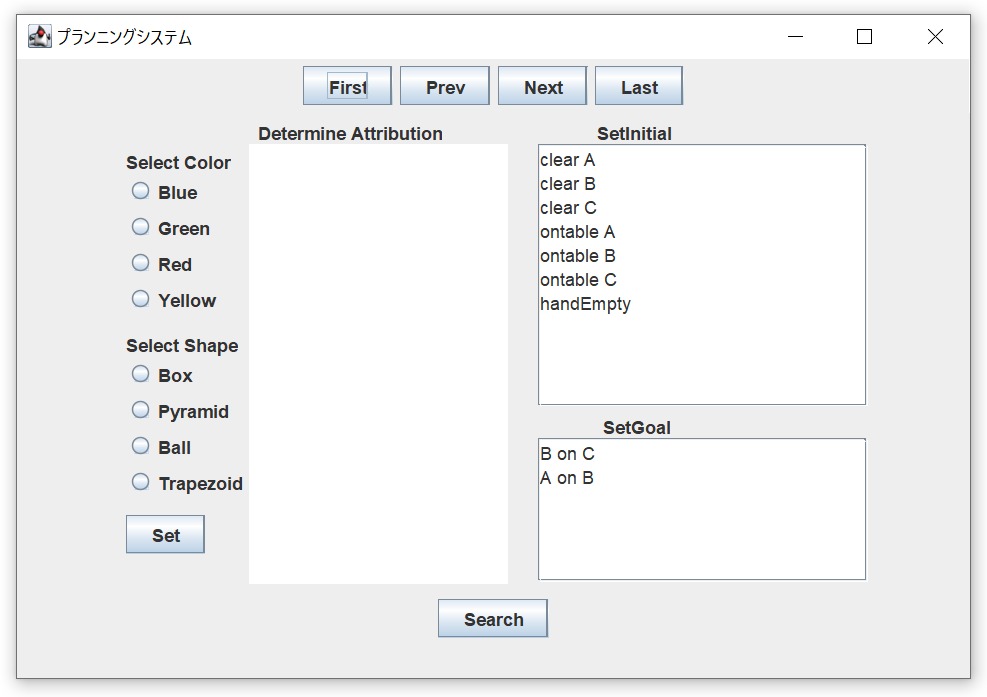
\includegraphics[scale=0.6]{images/page1.PNG}
    \caption{初期状態と目標状態,属性の決定画面}
    \label{fig:page1}
  \end{center}
\end{figure}
\clearpage
初めに実行を行った段階で,デフォルト状態でのプランニングが行われているため,ページ上部のNextボタンを押すと次の画面に遷移し,ブロック操作の過程の描画画面となる.Nextボタンを押すと次の状態へ,Prevボタンを押すと一つ前の状態へ遷移する様子が確認できる.(図\ref{fig:page2},図\ref{fig:page3},図\ref{fig:page4}).\\
%\clearpage
\begin{figure}[htbp]
  \begin{center}
    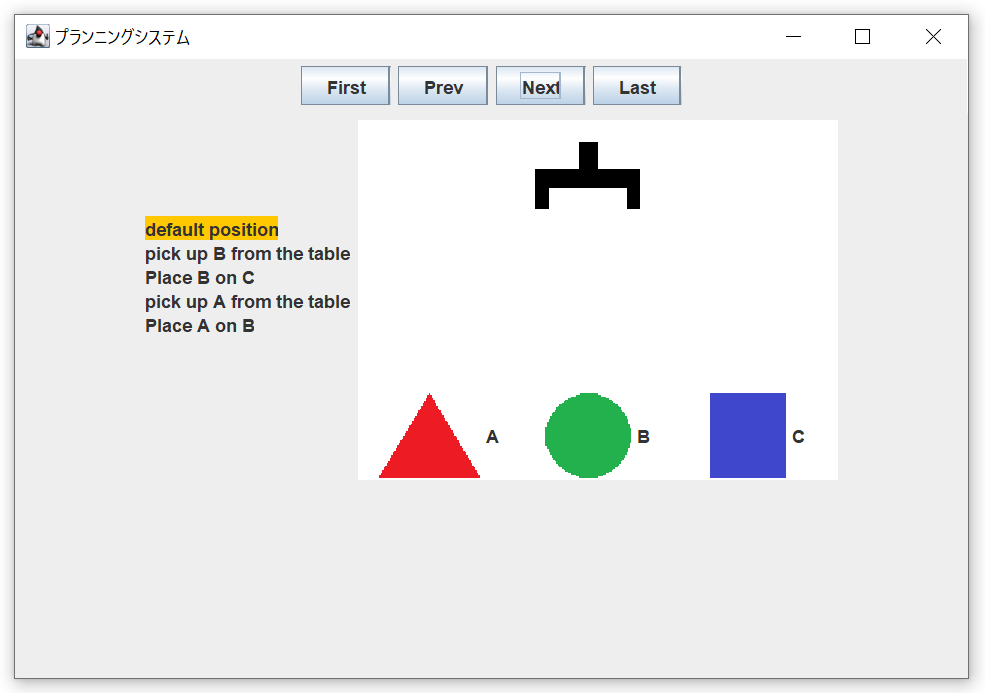
\includegraphics[scale=0.6]{images/page2.PNG}
    \caption{ブロック操作の過程1}
    \label{fig:page2}
  \end{center}
\end{figure}
%\clearpage
\begin{figure}[htbp]
  \begin{center}
    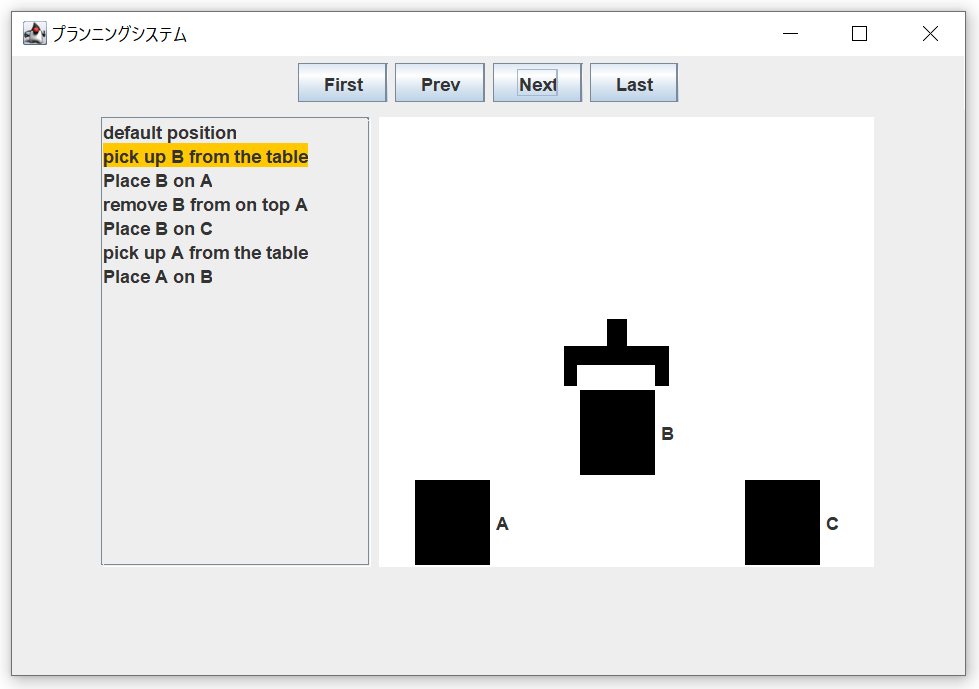
\includegraphics[scale=0.6]{images/page3.PNG}
    \caption{ブロック操作の過程2}
    \label{fig:page3}
  \end{center}
\end{figure}
%\clearpage
\begin{figure}[htbp]
  \begin{center}
    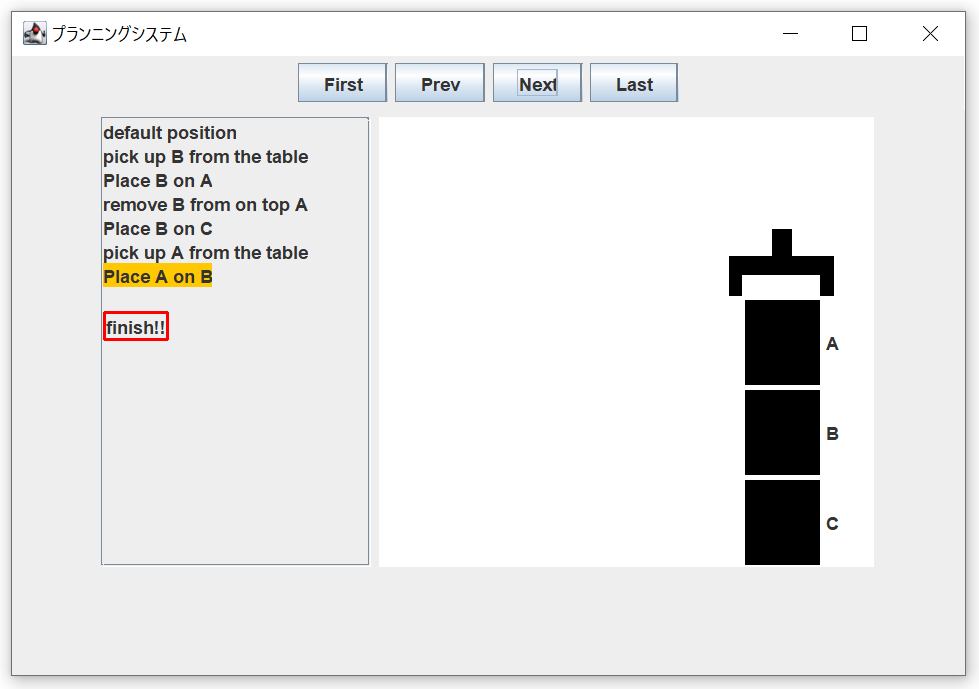
\includegraphics[scale=0.6]{images/page4.PNG}
    \caption{ブロック操作の過程3}
    \label{fig:page4}
  \end{center}
\end{figure}
\clearpage
さらに,Firstボタンを押すと一番初めの設定画面へ,Lastボタンを押すと一番最後の画面であるオペレータとプランニング結果を表す画面へと遷移する(図\ref{fig:page5}).\\
\begin{figure}[htbp]
  \begin{center}
    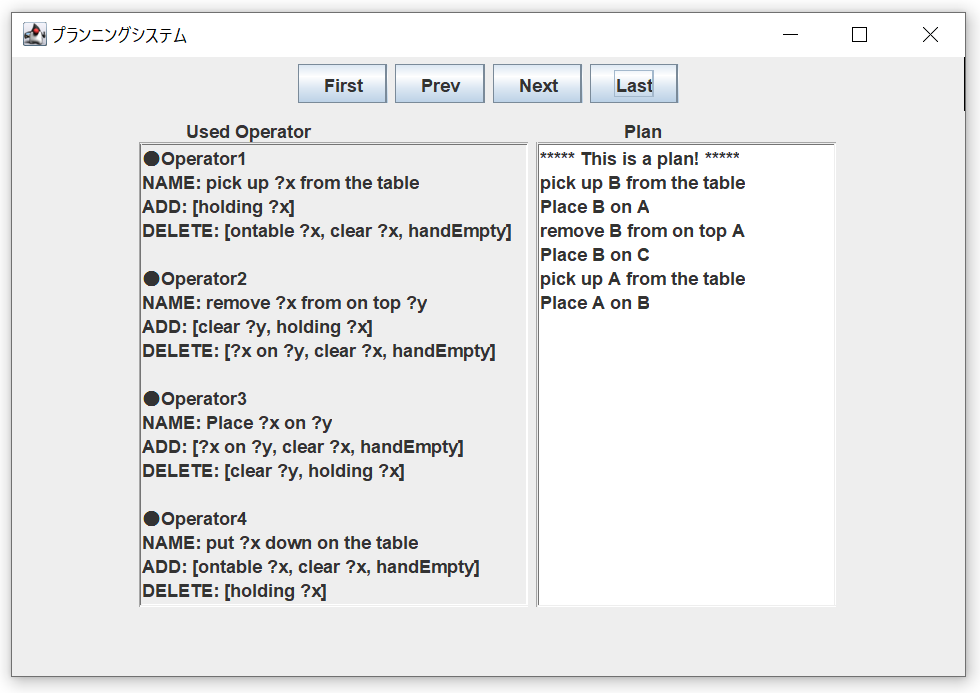
\includegraphics[scale=0.6]{images/page5.PNG}
    \caption{オペレータとプランニング結果の情報}
    \label{fig:page5}
  \end{center}
\end{figure}

\clearpage
次に,初期状態,目標状態,属性情報を変更してプランニングを行う.まず初期画面の左上に現在の属性情報があり,これを左下のラジオボタンを追加・削除・編集ボタンで変更する(図\ref{fig:page6}).\\

\begin{figure}[htbp]
  \begin{center}
    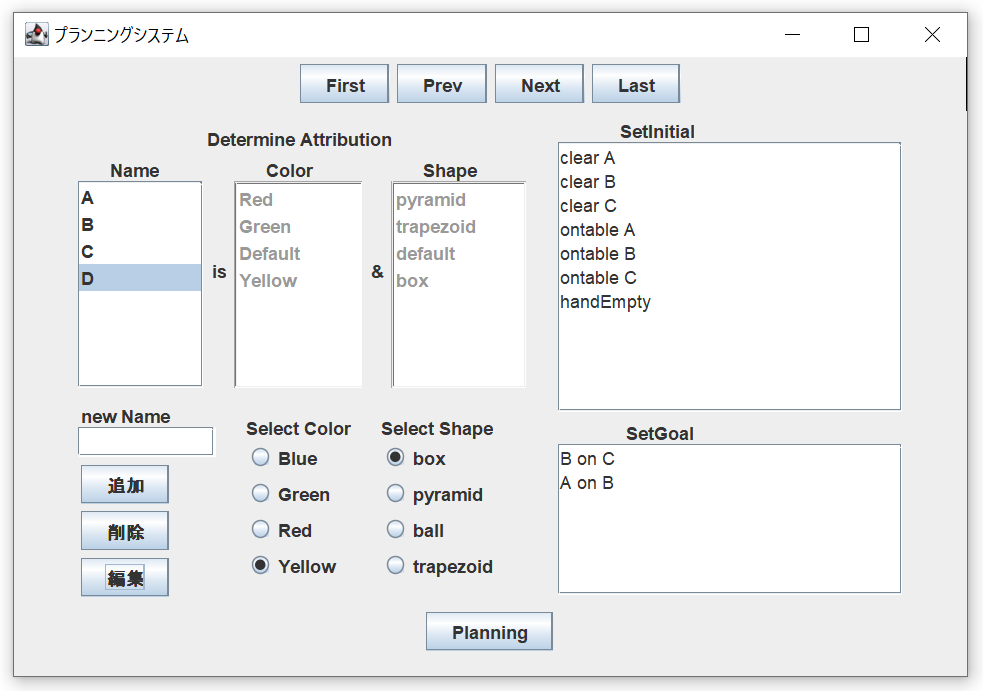
\includegraphics[scale=0.6]{images/page6.PNG}
    \caption{属性情報の変更}
    \label{fig:page6}
  \end{center}
\end{figure}
また,ブロック追加時には左下にある'new\ Name'欄に新規ブロックの名前を入力する必要があるが,無記入で追加をした場合や既にある名前を入力した際にはエラーメッセージがダイアログウィンドウで表示されるようになっている(図\ref{fig:page7},図\ref{fig:page8}).編集・削除ボタンを押した際に属性リストの名前を選択していなかった場合にも同様にエラーメッセージが表示される.\\
\begin{figure}[htbp]
  \begin{center}
    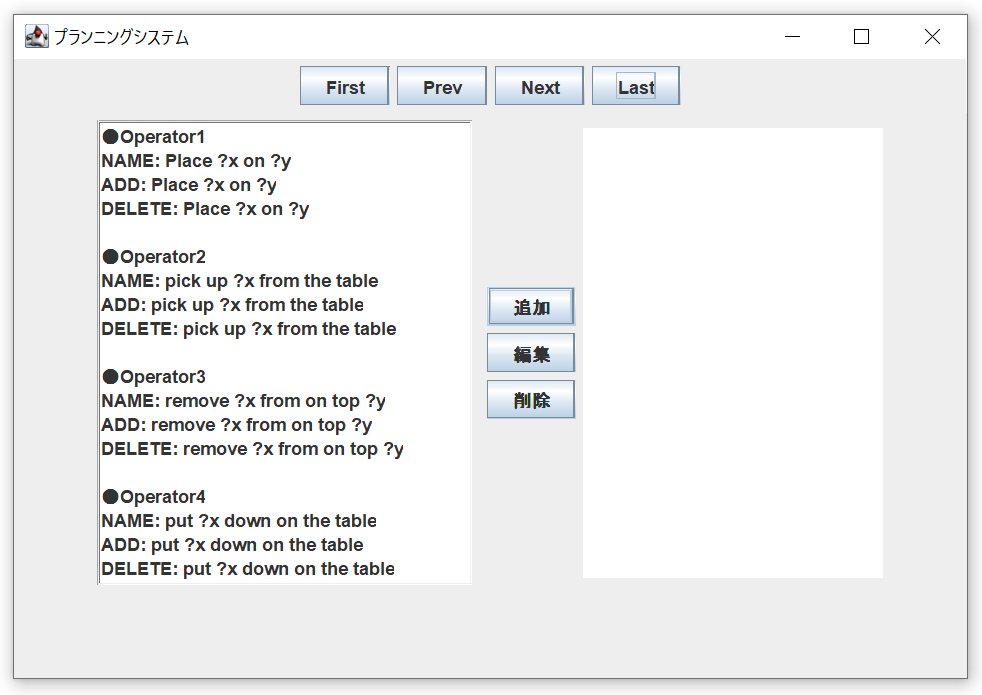
\includegraphics[scale=0.6]{images/page7.PNG}
    \caption{エラーメッセージの表示1}
    \label{fig:page7}
  \end{center}
\end{figure}
%\clearpage
\begin{figure}[htbp]
  \begin{center}
    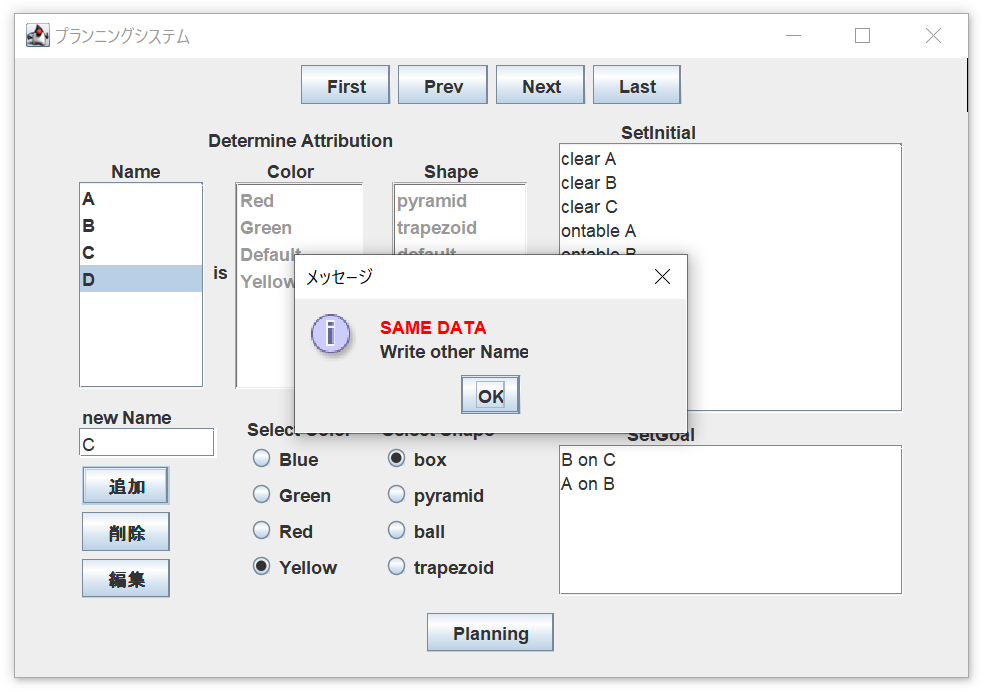
\includegraphics[scale=0.6]{images/page8.PNG}
    \caption{エラーメッセージの表示2}
    \label{fig:page8}
  \end{center}
\end{figure}
\clearpage
初期状態と目標状態の変更は初期画面の右側のテキストボックスに記述する形で行う.このとき,範囲を超えた記述をする場合はスクロールバーが表示される(図\ref{fig:page9}).また,属性情報変更時と同様に初期状態と目標状態に何も記入せずPlanningボタンを押すとエラーメッセージが表示される.\\
%\clearpage
\begin{figure}[htbp]
  \begin{center}
    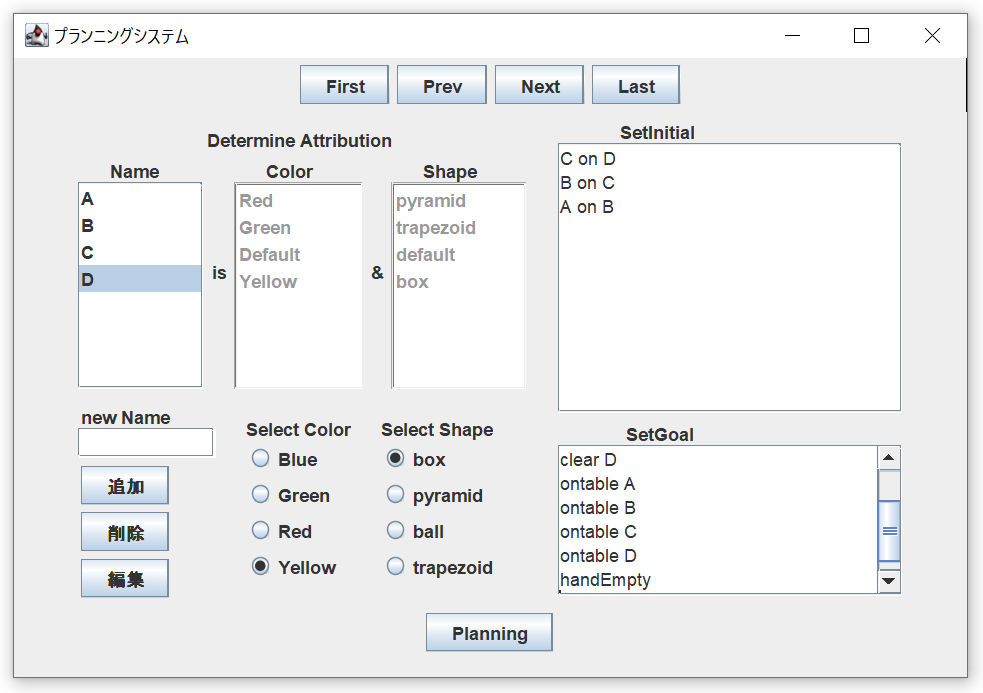
\includegraphics[scale=0.6]{images/page9.PNG}
    \caption{初期状態と目標状態の変更}
    \label{fig:page9}
  \end{center}
\end{figure}
\clearpage

変更を行った状態でPlanningボタンを押すと,定義した状態を基にプランニングが行われる.すると,探索が完了したことを伝えるメッセージが表示され,ブロック操作の過程の画面が新しく得られた結果が表示される.今回は例としてブロックを4つに増やし,属性情報を変えた(図\ref{fig:page10},図\ref{fig:page11},図\ref{fig:page12}).\\

\begin{figure}[htbp]
  \begin{center}
    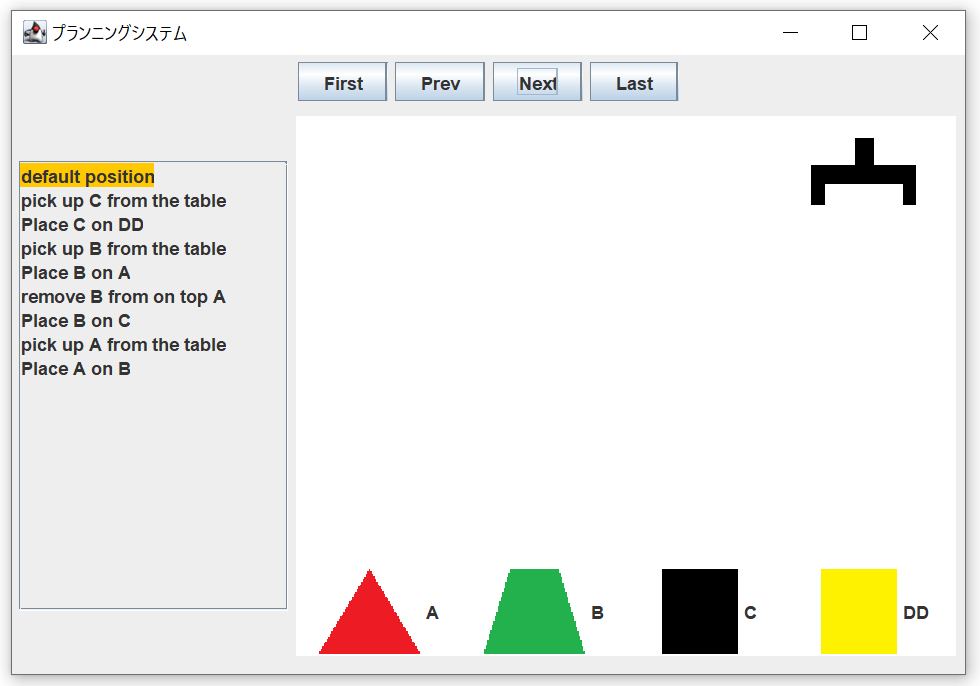
\includegraphics[scale=0.6]{images/page10.PNG}
    \caption{再実行時のブロック操作の過程1}
    \label{fig:page10}
  \end{center}
\end{figure}
%\clearpage
\begin{figure}[htbp]
  \begin{center}
    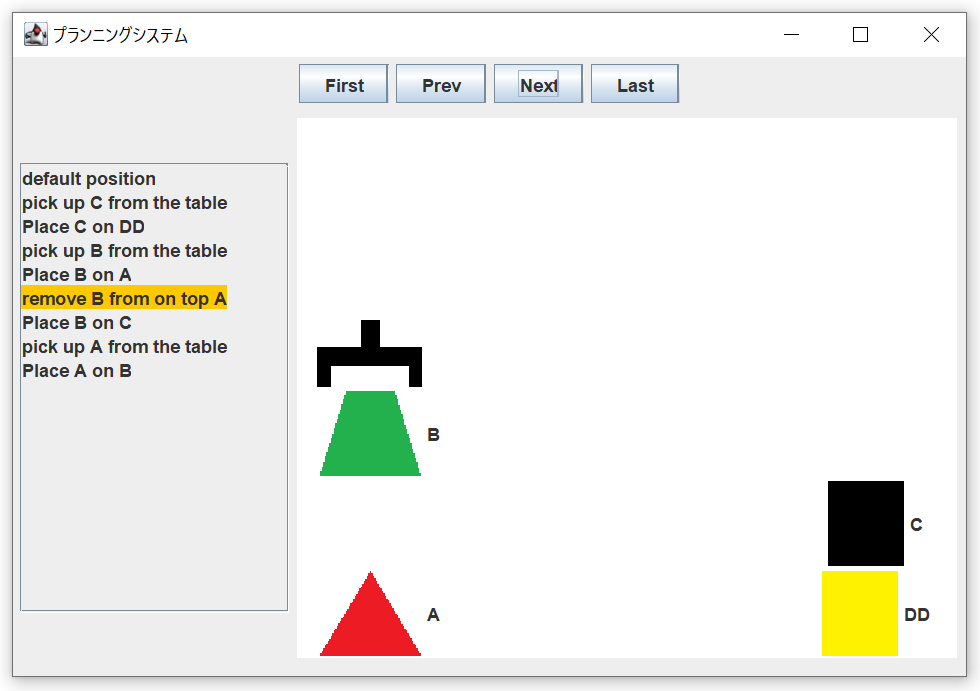
\includegraphics[scale=0.6]{images/page11.PNG}
    \caption{再実行時のブロック操作の過程2}
    \label{fig:page11}
  \end{center}
\end{figure}
\begin{figure}[htbp]
  \begin{center}
    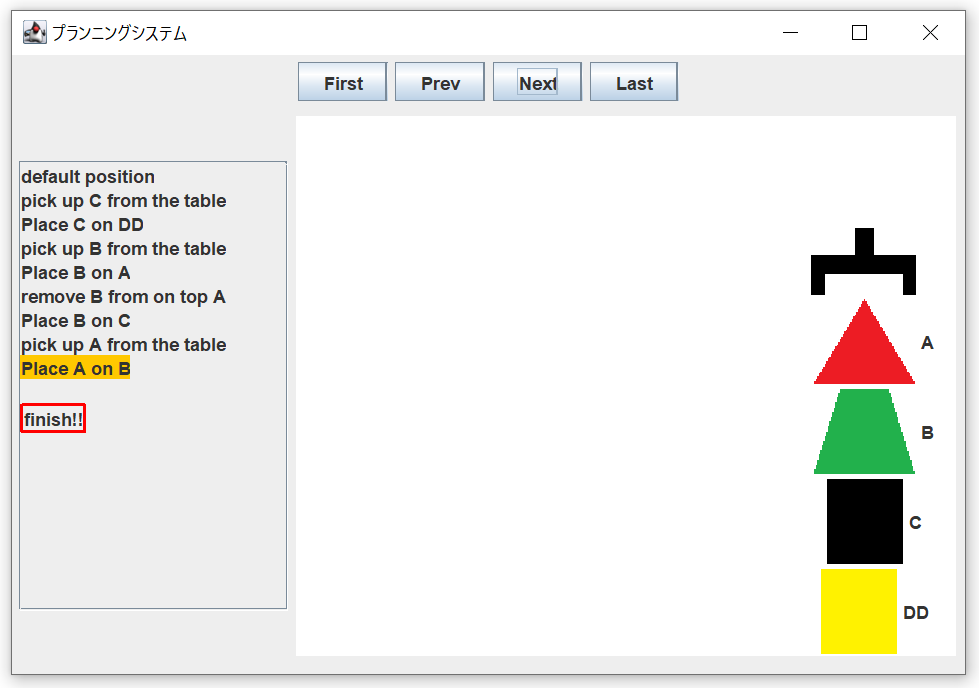
\includegraphics[scale=0.6]{images/page12.PNG}
    \caption{再実行時のブロック操作の過程3}
    \label{fig:page12}
  \end{center}
\end{figure}

\clearpage
またブロックを積み上げる動作だけでなく,ブロックをおろす場合もグラフィカルな可視化を行うことが出来る(図\ref{fig:page14},図\ref{fig:page16}).
\begin{figure}[htbp]
  \begin{center}
    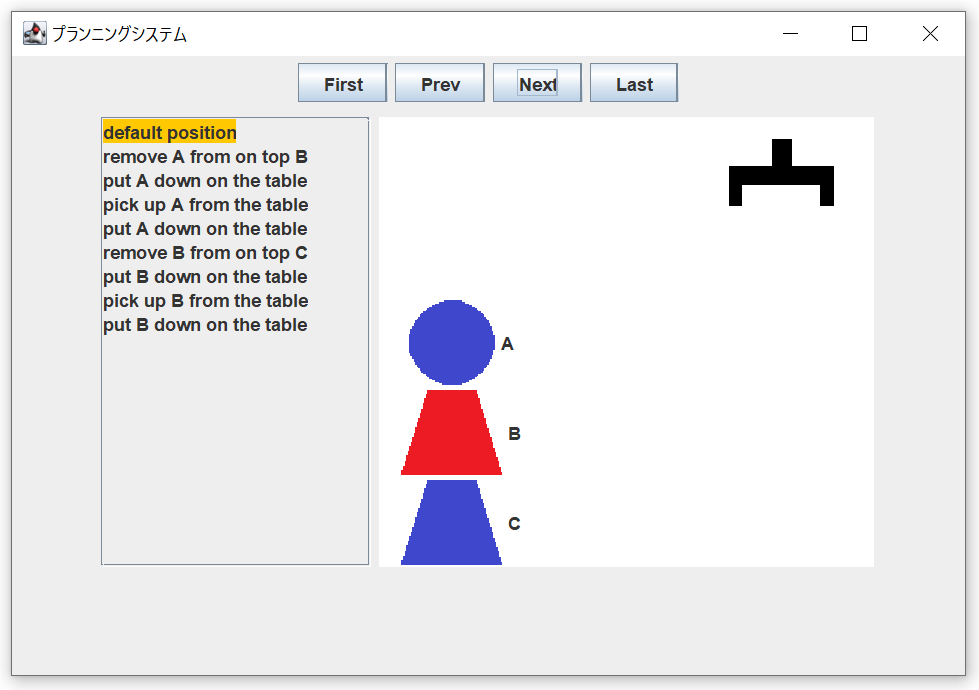
\includegraphics[scale=0.49]{images/page14.PNG}
    \caption{積み下ろしのブロック操作の過程1}
    \label{fig:page14}
  \end{center}
\end{figure}
%\begin{figure}[htbp]
%  \begin{center}
%    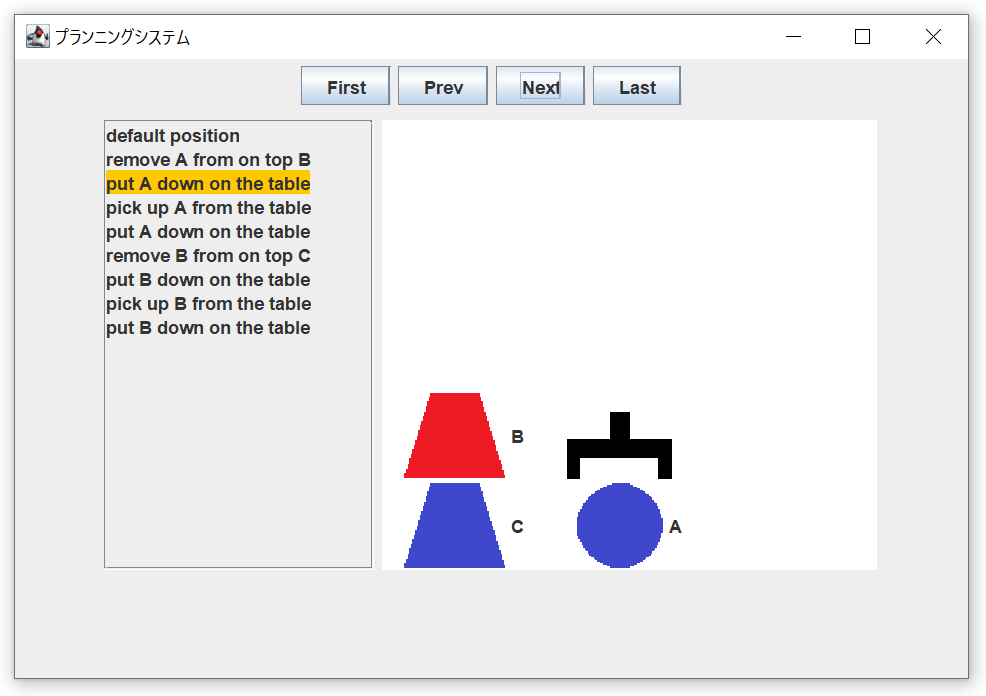
\includegraphics[scale=0.6]{images/page15.PNG}
%    \caption{積み下ろしのブロック操作の過程2}
%    \label{fig:page15}
%  \end{center}
%\end{figure}
%\clearpage
\begin{figure}[htbp]
  \begin{center}
    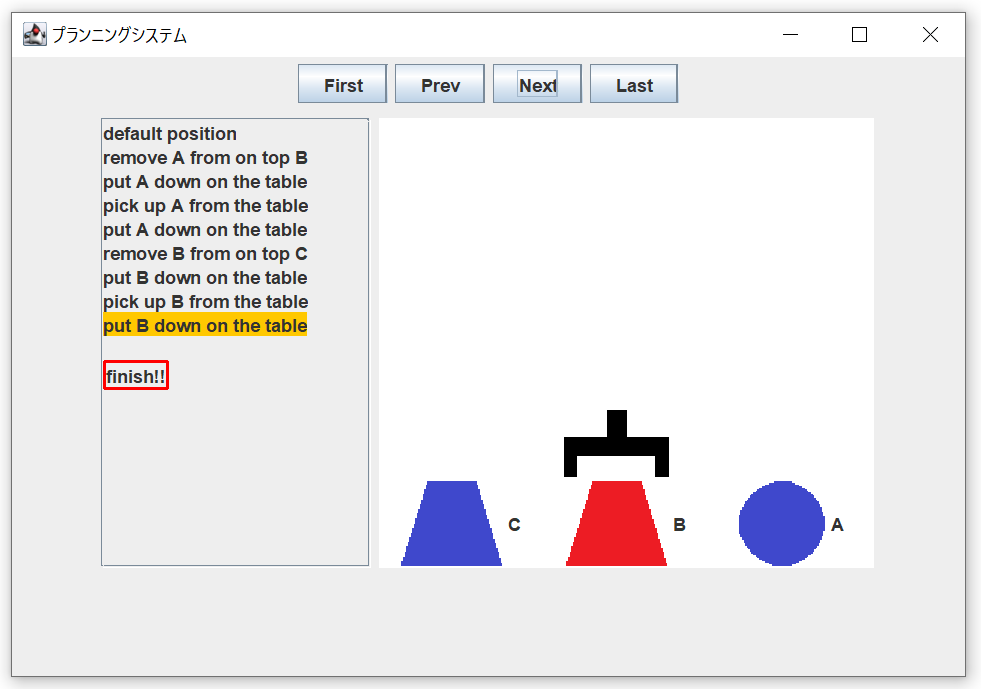
\includegraphics[scale=0.49]{images/page16.PNG}
    \caption{積み下ろしのブロック操作の過程2}
    \label{fig:page16}
  \end{center}
\end{figure}

\clearpage
次に,初期状態と目標状態が同一であった場合の動作を示す.初期状態を示す画面の後に以下の表示が現れ,既に目標状態にあることが示される(図\ref{fig:page17}).
\begin{figure}[htbp]
  \begin{center}
    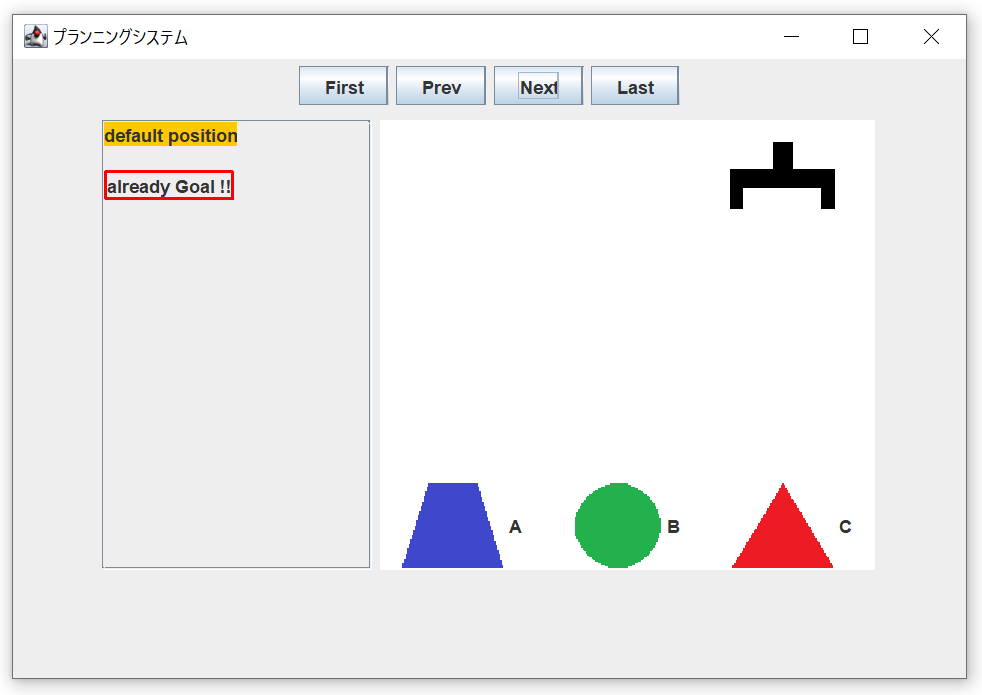
\includegraphics[scale=0.6]{images/page17.PNG}
    \caption{初期状態と目標状態が同一の場合}
    \label{fig:page17}
  \end{center}
\end{figure}

さらに,禁止制約によってプランニングが行えなかった場合の動作を示す.Planningボタンを押すと,プランニングが行えなかったことを示すエラーメッセージが表示され,ユーザーが定めた属性情報・禁止制約・ユーザーが定めた目標状態が表示される(図\ref{fig:prohibit1},図\ref{fig:prohibit2}).\\

\begin{figure}[htbp]
  \begin{center}
    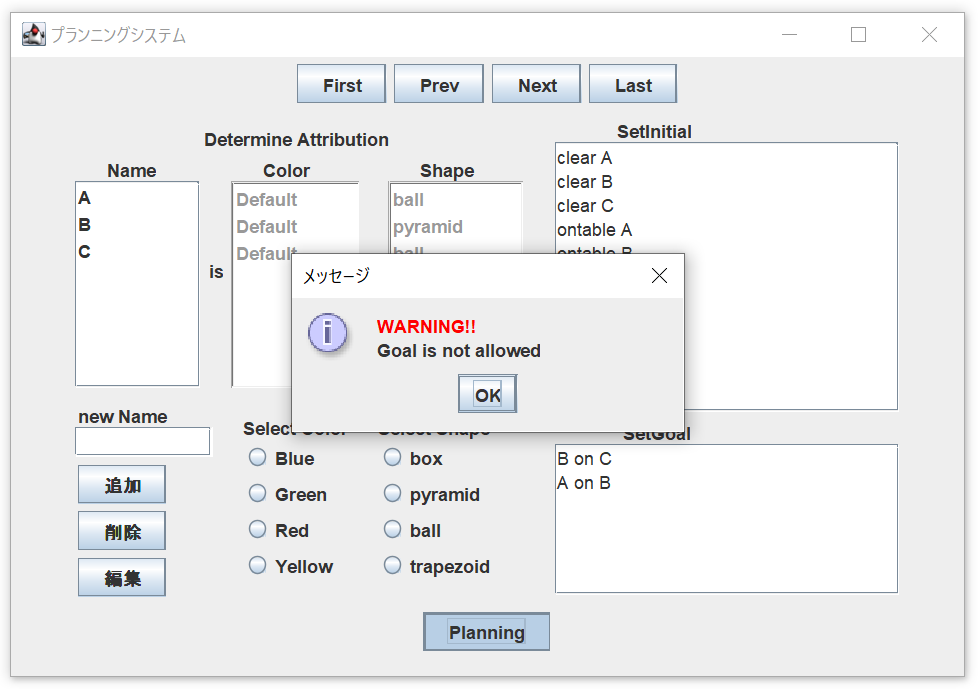
\includegraphics[scale=0.6]{images/prohibit1.PNG}
    \caption{禁止制約を示すエラーメッセージの表示}
    \label{fig:prohibit1}
  \end{center}
\end{figure}
\begin{figure}[htbp]
  \begin{center}
    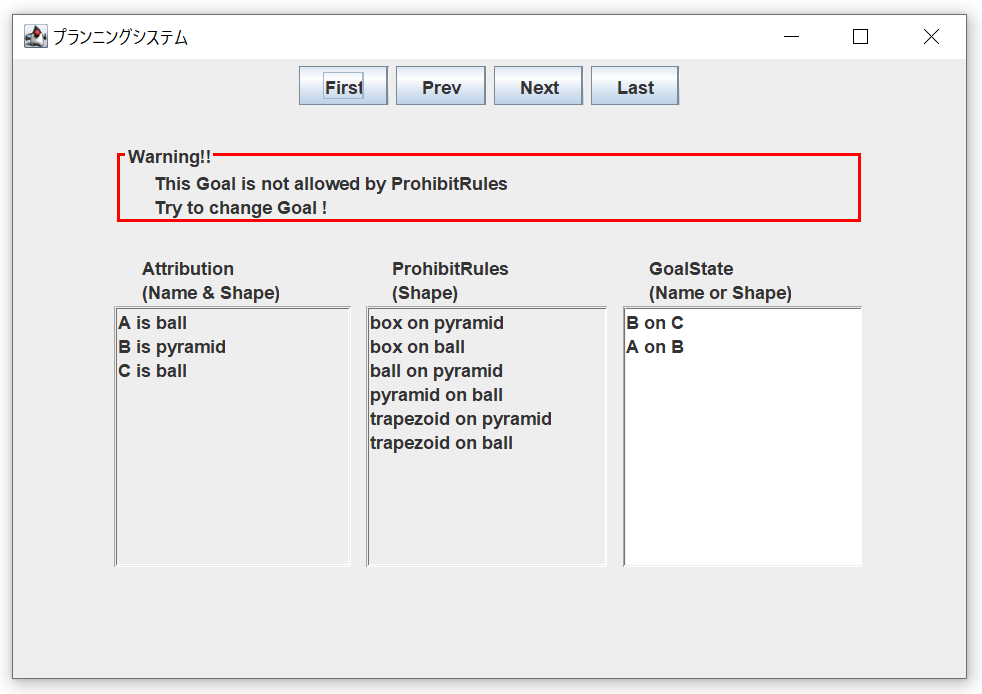
\includegraphics[scale=0.6]{images/prohibit2.PNG}
    \caption{属性情報・禁止制約・目標状態の表示}
    \label{fig:prohibit2}
  \end{center}
\end{figure}

\clearpage

\noindent (青山担当) \\
Presenter.javaのmainメソッドを実行したところ,以下のような結果が得られ,値が正しく取得できていることが分かる.

\begin{lstlisting}[caption=Presenterの実行, label=pres]
...
***** This is a plan! *****
pick up B from the table
...

-----on Presenter-----
[clear blue, clear green, clear red, ontable ball, ontable trapezoid, ontable box, ontable pyramid, handEmpty]
[trapezoid on box, ball on trapezoid]
pick up ?x from the table
{?x=B}
\end{lstlisting}

\subsection{考察}
\noindent (湯浅担当) \\
今回は新しい知識について学ぶ必要があったため,まず初めにプログラムを二週間という期間の中でどのように実装するかの計画を出来るだけ細かく立てた.これによっていつまでに何を終わらせておけば良いかが明確になり,スケジュール調整がし易くなったため,初めに分かる範囲で詳細な計画を立てることが重要であると分かった.\\

今回は状態遷移をグラフィカルに可視化するため,どのようにそれを描画するかがまず大きな課題であった.初めは一枚のフレームに状態遷移を全て表示することを考えていたが,それでは状態遷移が何回行われるか分からない今回の課題では表示方法に問題がある.そこで異なる方法を検討した.GUIについて調べる中で,CardLayoutを用いればカードの枚数を増やしていくことで状態の遷移回数の変化にも対応できると分かり,この実装でプログラムを考えた.\\

次に描画をどのように行うかについて考えた.GUI上での図形の描画は座標指定で行う必要がある.しかしこれではレイアウトマネージャーを無効にする必要がある.この場合描画を全て自身の座標管理で行わなければならないため,描画の難度が高いと考えた.そこで今回は図形を画像として予め作成しておき,これをImageIconとして取り込み,BoxLayoutで等分に分割した座標空間に対して割り当てていくことで実装を行うことを考えた.BoxLayoutを用いることで,空間の行と列を指定した数に等分に分割し,それぞれに画像を割り当てることが出来る.この方法を用いることで,座標指定をすることなく図形を配置でき,比較的容易に状態遷移を描画出来ると考えた.\par
しかしこの方法を用いると,取り込んだ図に対して操作を行うことは出来ないことが分かった.そのため,画像の上に重なるように図形の名称(A,B,C等)を入れることや,取り込んだ画像の色を上書きすることが出来ないため,今回は図形の横に名称を記載し,画像は色違いのものをはじめから用意しておくことでこの問題を解決した.\par
予め図形を作成しておくことから,図形や色の任意指定も出来なくなってしまった.しかし座標指定を行う場合も図形の任意指定はできないと考えられるため,図形の任意指定を行えるようにするためには異なる方法を検討する必要があると感じた.\\

また,表示範囲は図形の大きさと個数から定めることで,ブロックの個数の変化に対応できるようにした.この方法を用いることで,表示する個数が変化しても描画内容に大きな変化が起きないようになった.しかし初めに設定したフレームの大きさの関係で,5個以上のブロックの描画を行うと規定のフレームサイズを描画が超えてしまう.これにより,フレームをユーザー自身が大きくする必要が出てしまった.これについてはスクロールバーをつけることで対応しようと考えたが,実装が難しく実現できなかった.そのため描画は正しく行えたものの,表示方法に課題が残る結果となった.同時に,初めに作成するフレームのサイズも考えて決める必要があると分かった.\\

さらに属性情報の更新方法をどのようにするか考えた.属性情報では,名前・色・形を連動させ変更しなければならない.加えて任意での色や形の設定が出来ないため,これをラジオボタンで操作することとした.ここで項目を選択して編集を行えるとより使いやすくなると考え,JListを用いることを考えた.さらに名前・色・形をそれぞれ別のJListで表示することで,見やすい表示を心掛けた.\par
しかし名前・色・形をそれぞれJListで管理すると,それぞれの項目を選択出来てしまうため,ユーザーが現在どの項目を編集しようとしているのかが分かりにくくなってしまう.これを解決するため色と形のJListは,プログラム側で編集を行う時以外は無効にすることで,ユーザーが操作できないようにすることを考えた.\\

また今回はユーザー視点の操作について考えた実装を心掛けた.\par
まず,ユーザーが任意で記述できる初期状態や目標状態・属性情報は記述スペースを超えた場合はスクロールバーが表示されるようにした.また出力される経路についても,表示画面よりも長くなってしまった場合はスクロールバーでの表示が出来るようにした.さらに状態遷移の描画を行う際の経路の表示では,自身がどの状態にあるのかを分かりやすくするため,現在の状態を表す一文に背景色としてオレンジ色を付けた.\par
経路が長くなってしまった場合はスクロールバーが表示されるものの,そのままでは常にスクロールバーが一番上にある状態でページが作成される.これでは表示範囲を超えた状態遷移のページでは,自身の現在の状態を確認するためにはスクロールバーを毎回下げる必要がある.これではユーザーにとって使い難いGUIだと考え,常に現在の状態が見える位置に来るように表示する座標位置を順に下げ,ユーザーがスクロールバーを動かさずに現在の状態を確認できるよう実装を行った.\par
さらに禁止されている入力を行った場合などはメッセージを表示することで,何が問題でどのようにすれば良いのかを分かりやすく示せるようにした. \\

\noindent (青山担当) \\
今回,Presenter側では特にやることがなく,GUI側の負担が大きいように感じた.しかし,GUI制作経験のある身として,可能な限りGUIが扱いやすいようなPresenterとなるよう心がけた.例えば,プランの過程の渡し方は,Operatorを少し書き加えて実現したことで,変数束縛も簡単に一緒に取得できるようにしたことや,String型でも過程を受け取れるようにしたことでGUI側で行うべき処理を減らせるようにしたことである.

しかし,今回の課題も前回同様最初はどのような形で値を渡すかで悩むこととなった.前回よりも早く意識のすり合わせと進捗の説明を担当者間で共有できたため,今回はよりスムーズに実装に漕ぎ着けたのだと考えられる.

また,GUIとPresenterの分担を交代してやってみることで,GUIの面ではレイアウトの仕方や表示のための工夫,Presenterの面ではPlanner等の元のプログラムから途中のデータを引き継いだり引き渡すことの難しさやすべき考慮等を学ぶことができた.このように,ある程度経験がついた状態で役割を大胆に変えてみることは,お互いのプログラミングスキル向上を促進し合える一つの手だと考えられる.


\section{発展課題5-5}
\begin{screen}
    ブロックワールド内における物理的制約条件をルールとして表現せよ.
    例えば,三角錐(pyramid)の上には他のブロックを乗せられない等,その世界における物理的な制約を実現せよ.
\end{screen}
\subsection{手法}
ブロックワールド内における物理的制約条件(以下、禁止制約と表現する)をルールとして表現し,プランニングに反映するために,
課題5-3で作成した属性に関する処理を扱うクラスAttributions内に禁止制約のルールを保持させる方法を考案した.
例えば,"box on pyramid"(三角錐の上に正四面体がある)のようなルールが物理法則に反する禁止制約に当たる. \\
これらの禁止制約のルール集合を,課題5-3で結びつけた「属性とブロックの関係」をもとに,属性を用いた表現からブロックによる表現に置き換える. \\
以上により,ゴールリストやオペレーター適用後の状態とブロックによって表現される禁止制約を比較することで,
物理法則に反する状態を削除することができる.
また,ゴールリストに物理法則に反するものが含まれる場合には,ゴール不成立とする. 

以下に,今回実装した禁止制約の例を示す. \\

\begin{figure}[!hbt]
  \centering
  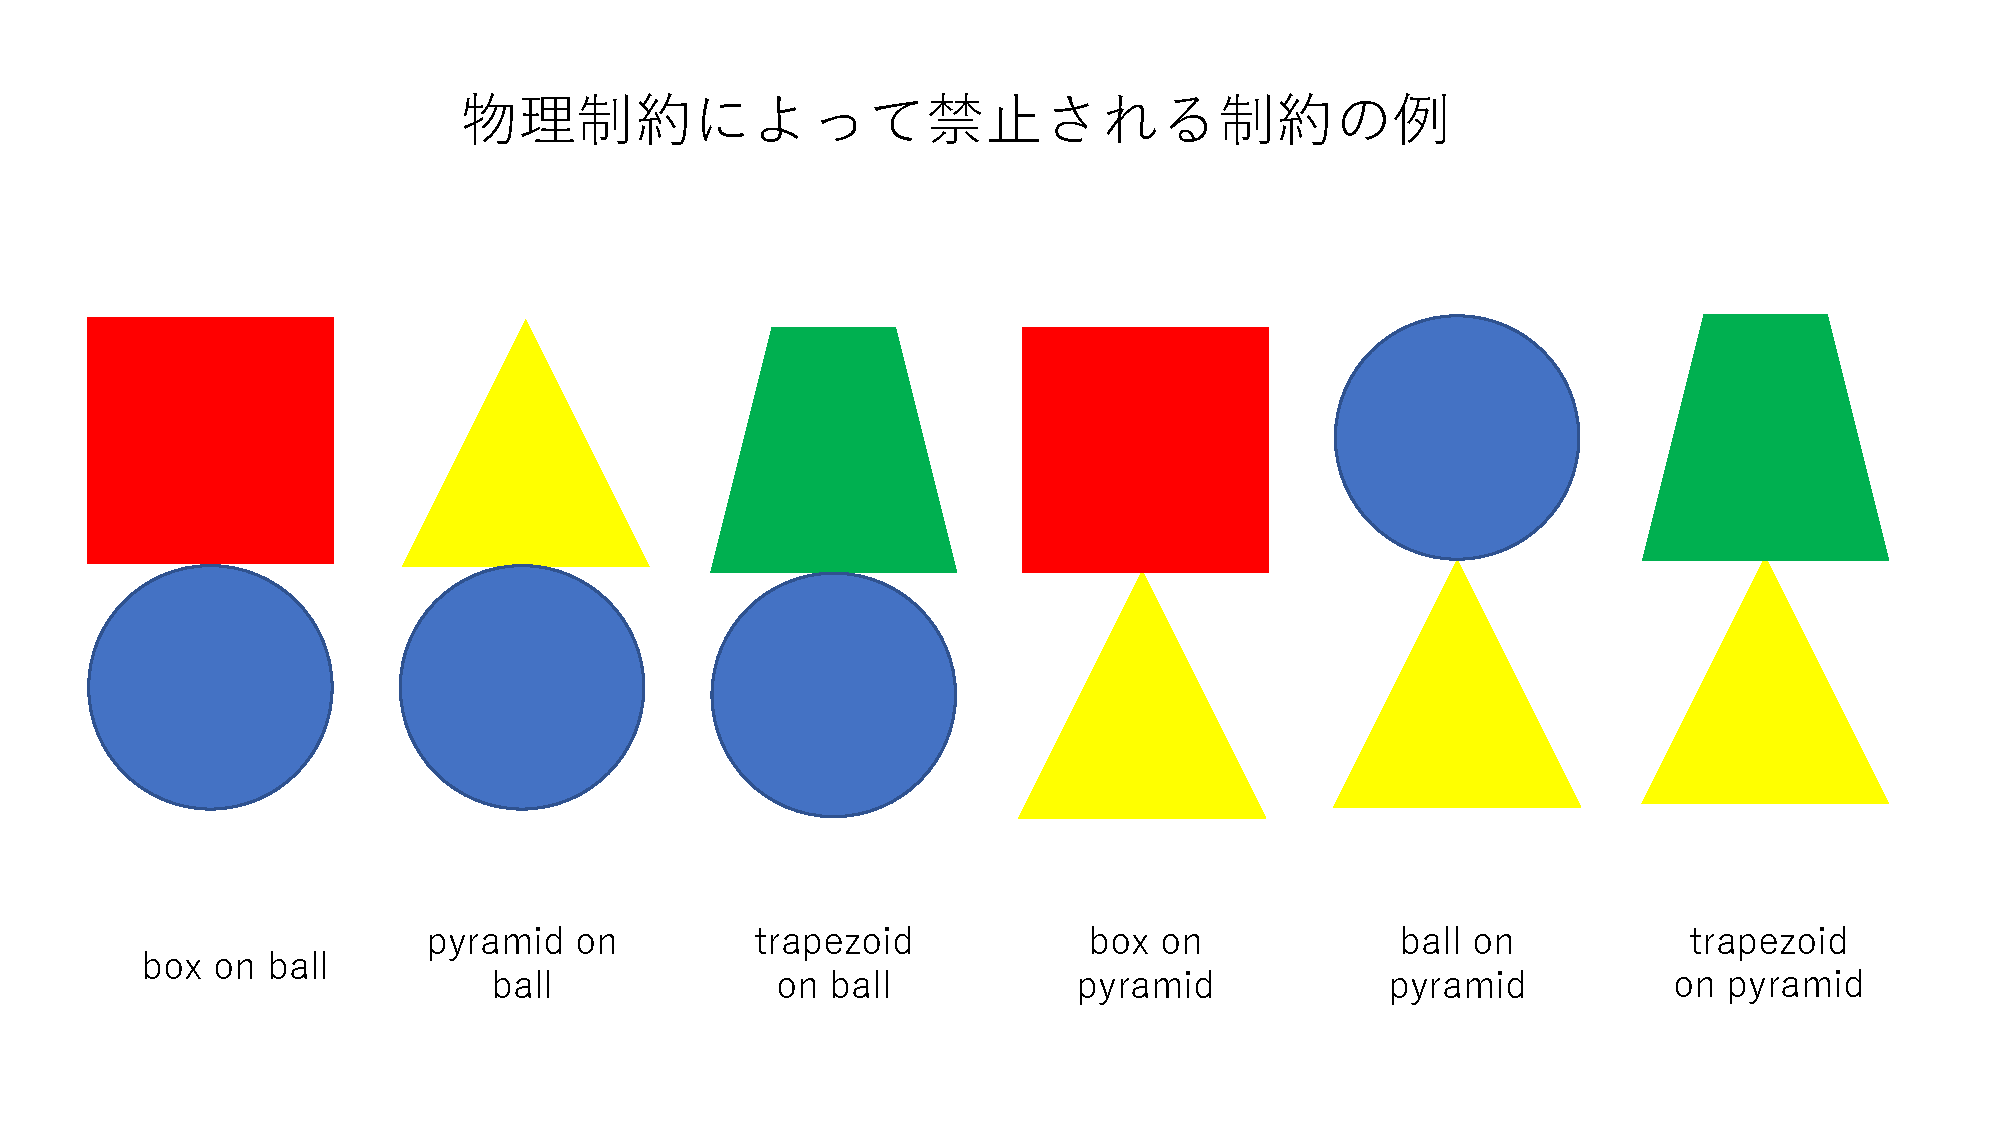
\includegraphics[scale=0.35]{images/prohibit-rules.pdf}
  \caption{物理制約によって禁止される制約の例}
\end{figure}

\subsection{実装}
まず,属性を扱うAttributionsクラス内にArrayList<String>型の禁止制約のルール集合prohibitRulesを保持させる.
このprohibitRulesはコンストラクタから呼び出されるメソッドaddProhibitRules()により禁止制約のルールが追加される. \\
加えて,属性によって表現された禁止制約のルールをブロックによる表現に置き換えたルール集合prohibitBlockStatesも定義する.
prohibitRulesからprohibitBlockStatesに変換を行うに当たっては,課題5-3で作成したメソッドeditStatementListを用いる. \\
次に,状態と禁止制約を比較するメソッドcheckProhibitBlockState(String state)を実装した.
このメソッドを以下に示す.
\begin{lstlisting}[caption=checkProhibitBlockStateメソッドの実装, label=mid]
    private Boolean checkProhibitBlockState(String state) {
		for(String prohibitBlockState: prohibitBlockStates) {
			if(prohibitBlockState.equals(state)) {
				System.out.println("【Warning!:状態"+state+"は禁止制約です!!】");
				return false;
			}
		}
		return true;
	}
\end{lstlisting}
2~7行目に渡って,全ての禁止制約のルール集合の要素と仮引数で受け取った状態を比較する処理を行なっている.
ここで,一つでも禁止制約と一致すると,falseが返却される.
反対に,全ての禁止制約と一致しなかった場合には,trueが返却される. \\
続いて,このcheckProhibitBlockStateメソッドを利用するcheckStates(ArrayList<String> states)メソッドの説明を行う.
このメソッドについても以下に示す.
\begin{lstlisting}[caption=checkStatesメソッドの実装, label=mid]
    ArrayList<String> checkStates(ArrayList<String> states) {
		ArrayList<String> checkedStates = new ArrayList<String>();
		for(String state: states) {
			if(checkProhibitBlockState(state)) {
				checkedStates.add(state);
			}
		}
		return checkedStates;
	}
\end{lstlisting}
3~7行目に渡って,仮引数で受け取った状態集合の各要素をcheckProhibitBlockStateの引数として渡すことで,禁止制約のチェックを行なっている.
結果としてtrueが帰ってきた場合にはチェック済みの状態集合checkedStatesに格納し,falseの場合には格納されない. \\
全ての要素のチェックが終わると,checkedStatesを返却する. \\
checkedStatesメソッドを,変化直後の状態集合に対して使用することによって,物理法則に反する状態を削除することができる.
以上の実装により,禁止制約のブロックワールドへの反映を実現した.

\subsection{実行例}
以下に,CUI上での実行結果を示す.
ただし,コンストラクタはデフォルトコンストラクタを使用するものとする.
\begin{lstlisting}[caption=禁止制約によりゴールが成立しなくなった場合, label=mid]
    ~/Programming2/Work5
    ●java Planner                                                                                                                                                                                                    【 feature/prohibit-rules 】
    ###### Add prohibitRule ######
    ****** ProhibitRule:box on pyramid ******
    ****** ProhibitRule:box on ball ******
    ****** ProhibitRule:ball on pyramid ******
    ****** ProhibitRule:pyramid on ball ******
    ****** ProhibitRule:trapezoid on pyramid ******
    ****** ProhibitRule:trapezoid on ball ******
    ++++++ EditStatement ++++++
    box on pyramid =====> A on B
    box on ball =====> A on C
    ball on pyramid =====> C on B
    pyramid on ball =====> B on C
    trapezoid on pyramid =====> trapezoid on B
    trapezoid on ball =====> trapezoid on C
    ========== goal:green on ball ==========
    ========== goal:blue on pyramid ==========
    ++++++ EditStatement ++++++
    green on ball =====> B on C
    blue on pyramid =====> A on B
    【Warning!:状態B on Cは禁止制約です!!】
    【Warning!:状態A on Bは禁止制約です!!】
    ---------- initInitialState:clear blue ----------
    ---------- initInitialState:clear green ----------
    ---------- initInitialState:clear red ----------
    ---------- initInitialState:ontable box ----------
    ---------- initInitialState:ontable pyramid ----------
    ---------- initInitialState:ontable ball ----------
    ---------- initInitialState:handEmpty ----------
    ++++++ EditStatement ++++++
    clear blue =====> clear A
    clear green =====> clear B
    clear red =====> clear C
    ontable box =====> ontable A
    ontable pyramid =====> ontable B
    ontable ball =====> ontable C
    handEmpty =====> handEmpty
    禁止制約によってゴールが成立しなくなりました
\end{lstlisting}
はじめに,3~9行目で禁止制約のルールがprohibitRulesに追加されている.
次に,10~16行目でeditStatementListによって属性による表現からブロックによる表現に変換されている.
17,18行目で属性表現によって指定されたゴールが19~21行目でブロックによる表現に変換されている. \\
そして,22,23行目で禁止制約がゴールに使用されていることが検出されている.
詳しく見てみると,22行目の検出は14行目と20行目の変換結果が一致することによるものであり,
23行目の検出は11行目と21行目の変換結果が一致することによるものである.
これらによって,ゴールリストに物理法則に反するものが含まれていることが判明したため,39行目においてメッセージが表示され,プランニングが終了している.

\subsection{考察}
課題5-3の実装をもとに禁止制約をブロックワールドに反映する実装を行なった.
特に,editStatementListのように再利用することのできるメソッドを作成したことは大きなプラスとなった.
また,課題5-3で取り決めた,属性をブロック名に置き換えてからプランニングを行う方針は,
課題5-5を進めるに当たって大きな助けにもなった.
具体的には,"A is red","A is pyramid","B is blue","B is ball"のようなルールのもと,
"pyramid on ball"のような禁止制約があるとする.
このとき,"red on blue"が状態に含まれるとき,属性表現のままプランニングを行うと見逃してしまうことになるが,
先に状態と禁止制約の属性表現をブロック名に変換して,"A on B"とすることによって,
物理法則に反する状態であると判定することができる. \\
したがって,課題5-3で取り決めた方針によって,課題5-5のプログラムの質を向上させることができたと考えている. \\
以上より,より良い実装を目指すに当たって,あらかじめ頭の中でプログラムの構造や処理の手順を考えておくことは非常に効果的であると感じた.


\section{発展課題5-6}
\begin{screen}
    ユーザが自然言語(日本語や英語など)の命令文によってブロックを操作したり,初期状態/目標状態を変更したりできるようにせよ.
    なお,命令文の動詞や語尾を1つの表現に決め打ちするのではなく,多様な表現を許容できることが望ましい.
\end{screen}

\subsection{手法}
ユーザの命令によるブロック操作を行う際, 何も考えずにただ漠然とブロックを動かしていては, プランニングの意味をなさない. 例えば「ブロックをA, B, Cの順に上から積んでいく」という目標が設定されている場合, オペレータは「Cの上にBを置く」のちに「Bの上にAを置く」とするのが理想であり, プランニングではその処理を行えなければならない. ここでユーザが「Cの上にAを置く」などでたらめなことをしてしまっては, プランニングの意味がない. そのため, ここにおける"ユーザによるブロック操作"の定義を, "プランニングを行っているユーザによるブロック操作"とする. \\
具体的には, プログラムが"おすすめ"の操作をユーザに知らせる. ユーザはそのおすすめを参考に処理を選択し, 実行する. もちろんユーザはプランニングを行っているという仮定のもとでの話なので, 条件に合わないオペレータ選択(つまり, 現在の目標に関わる内容がオペレータのAdd-listに存在しない)場合は, そのユーザの選択はプランニングにそぐわないとして実行されず, 代わりにおすすめの処理が行われるとする.\\
プログラムが勧める"おすすめ"のオペレータとは, 課題5-2で行った競合解消戦略によるオペレータ選択の内容である.\\
​
​
ここで問題となるのは, オペレータを4つの中から選択できたとしても, 中身までは選択できない.上記の例をもう一度考えると, 副目標「B on C」に対して, 「Place B on C」という内容はできても, 「Place A on C」という処理は, 行えない. \\
​
​
ブロック操作における競合解消戦略として, 教科書のプログラムではランダム関数を用いたオペレータの選択をしているが, その選択を適切に変える. 以下の2つの操作を試みている.
​
\begin{enumerate}
\item 推論の最中にユーザーの入力により, オペレータをその都度選択していく
\item ゴール状態と現在の状態を比べてより最適なオペレータを選択する
\end{enumerate} 
​
この推論システムは大きく, plannnigメソッドとplannigAGoalメソッドを再帰的に呼び合うことで成り立っている.
以下の図1を参考にしてほしい.
\begin{figure}[htbp]
 \begin{center}
  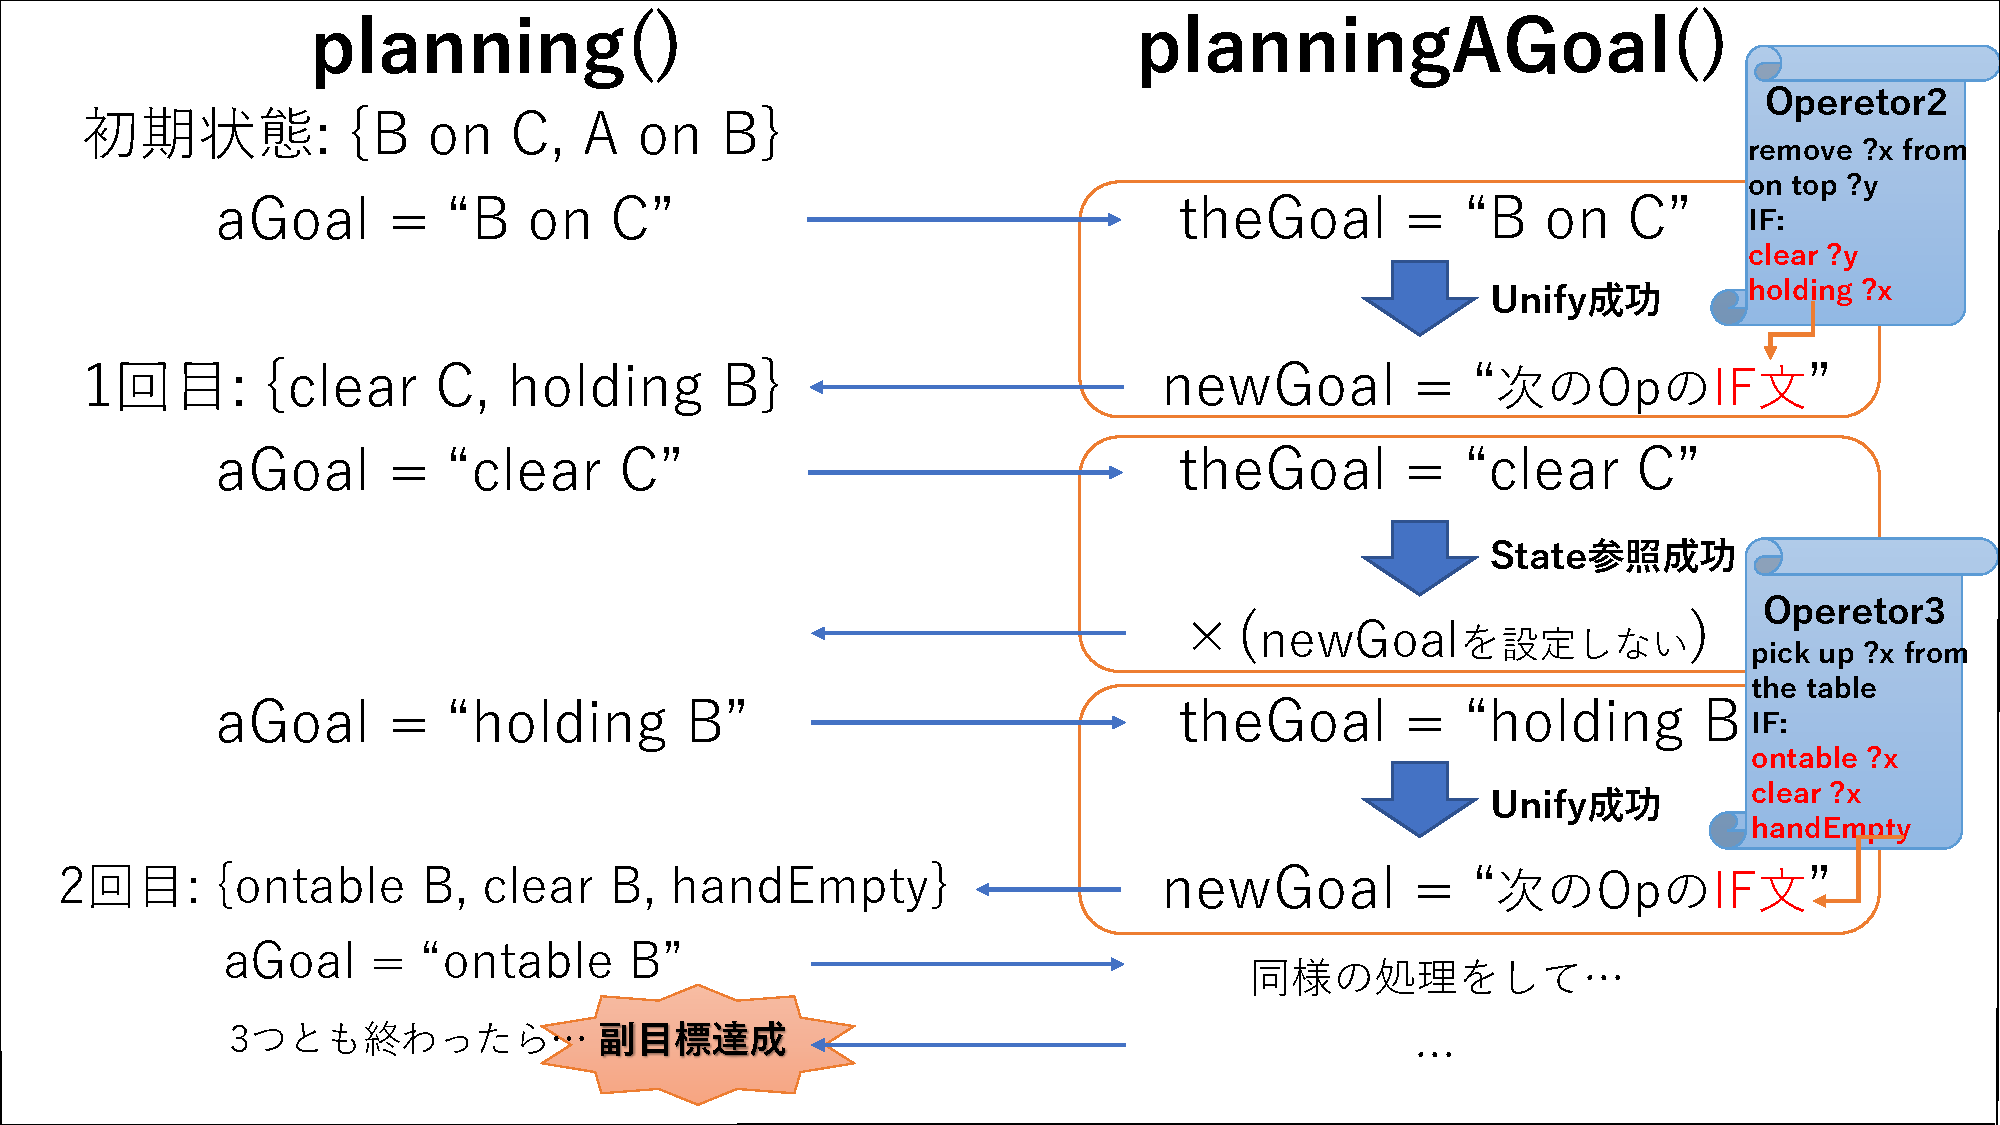
\includegraphics[width = 12cm, pagebox = cropbox, clip]{images/planning.pdf}
 \end{center}
 \caption[]{plannnigにおける相互メソッドの再帰構造}\label{fig:fig1.1}
\end{figure}
​
plannningAGoalメソッドで, plannnigメソッドから1つ取り出された目標状態を見て, 現状態に含まれていなければ各ルールのAdd-listからUnifyできるオペレータを,  現状態に含まれていればそのまま次の目標へといった流れである. このplanningAGoalメソッドでルールを選ぶ方法をランダムから変えれば良いことが分かる.\\
​
ランダムにオペレータを選択する際に, 教科書のプログラムは選択したオペレーションを一度, リストから取り除き, その後リストの最後に格納しているが, それだと適切なオペレータを選択できない.
​
\begin{figure}[htbp]
 \begin{center}
  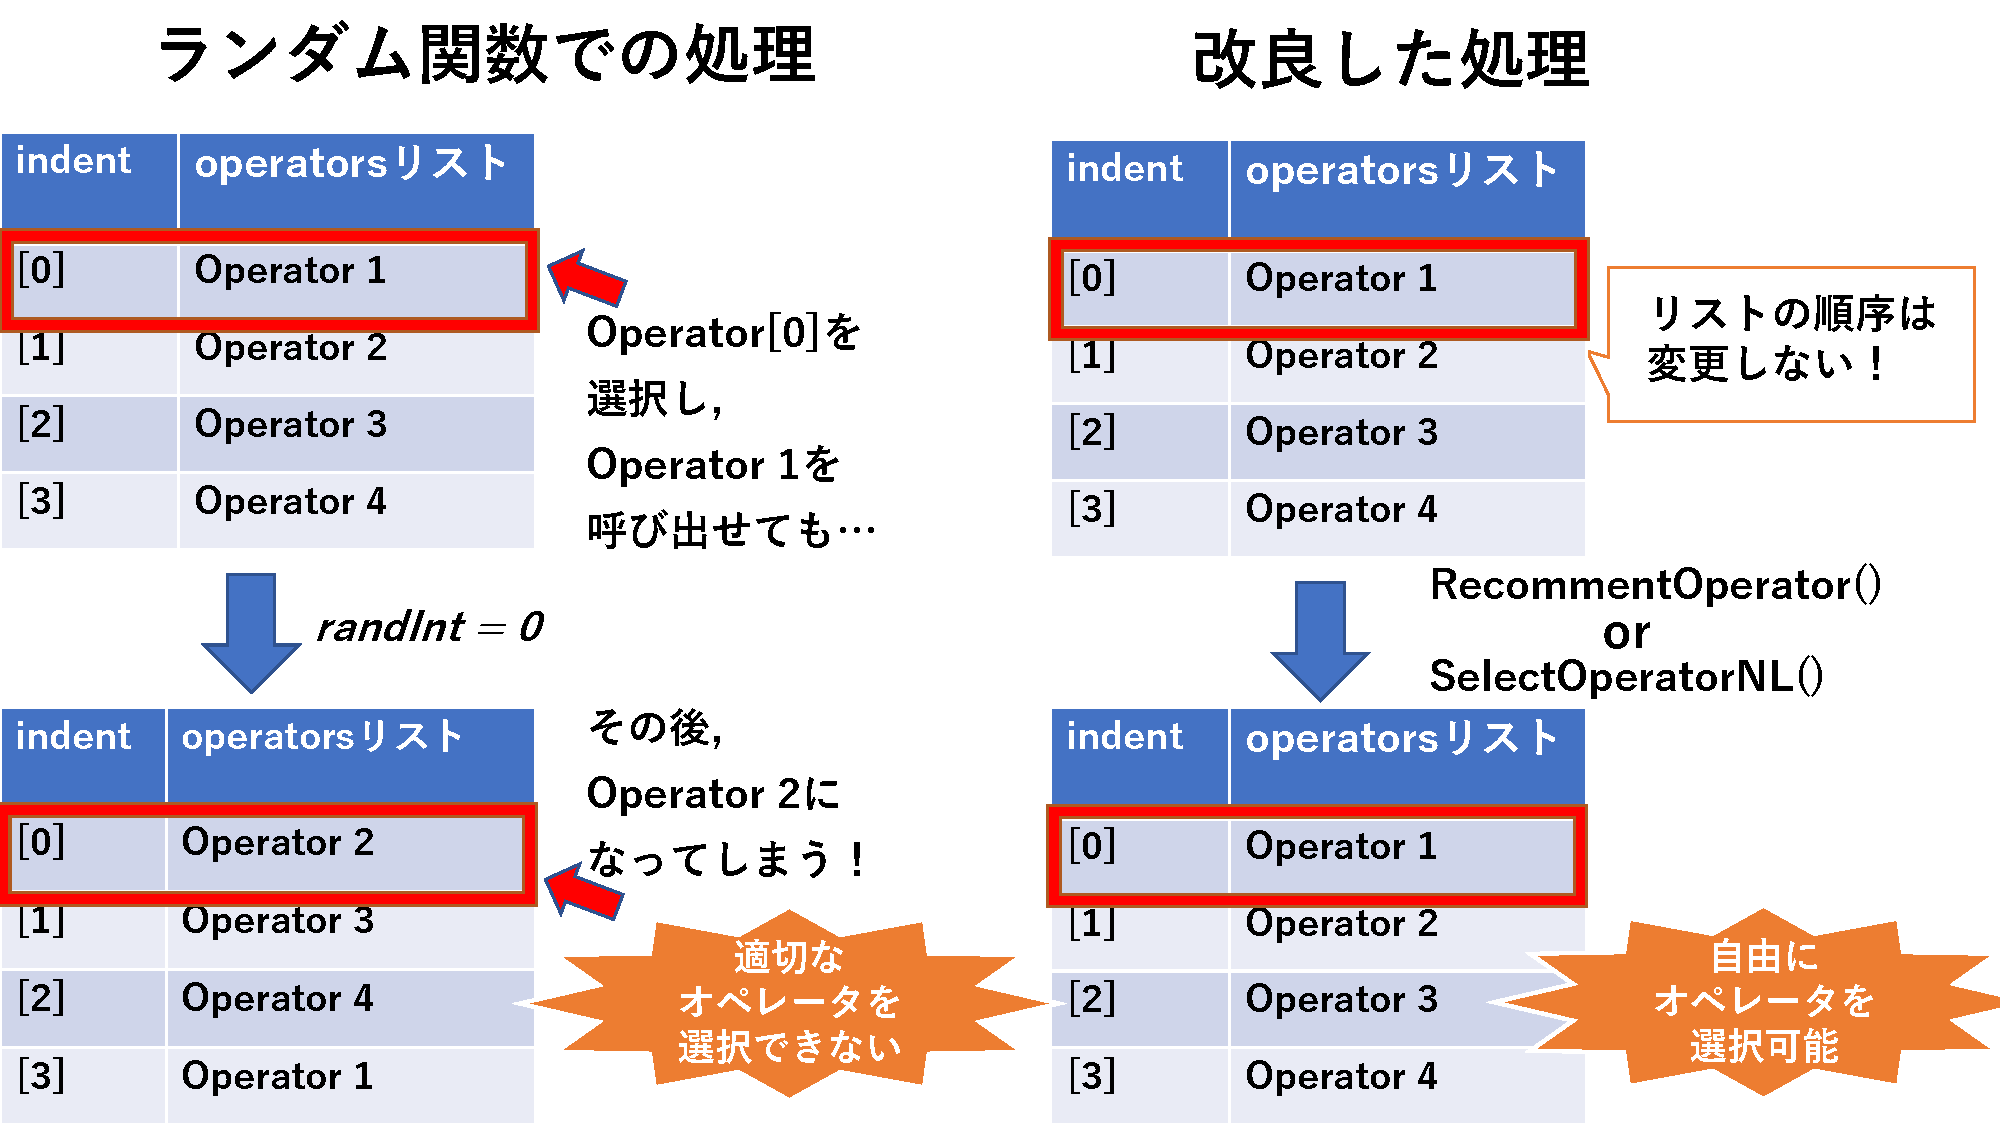
\includegraphics[width = 12cm, pagebox = cropbox, clip]{images/random.pdf}
 \end{center}
 \caption[]{operetarsリストの動き}\label{fig:fig1.1}
\end{figure}
​
そのため, 図2のように, operatorsリストの順序を適切に扱うことで, 自由にオペレータを選択, 取り出すことにする.
​
​
\subsection{実装}
planningAGoalメソッドにおけるオペレータの選択においては, それぞれ新しくメソッドを作成し, そこで適切なオペレータの番号を返すことになっている. 推論の最中にオペレータを選択するSelectOperetorNLメソッドと,, 最適なオペレータ選択をするReccomendOperetorメソッドを作成した.
\begin{lstlisting}[caption=オペレータ選択, label=src:No1]
	//1.ランダム用
	int randInt = Math.abs(rand.nextInt()) % operators.size();
  	Operator op = (Operator)operators.get(randInt);
	operators.remove(randInt);
	operators.add(op);
	//cPoint = randInt;
​
	//2.発展課題5-6用
	//int numOp = SelectOperatorNL();
​
	//3.その他開発用
	int numOp = RecommentOperator(theGoal);
​
	/* 2.3のどちらかを使うときは,このコメントアウトを外す!
	Operator op = (Operator)operators.get(numOp);
	System.out.println("オペレータ内容は = " + op.name);
	System.out.println("Thank you!");
	cPoint = numOp;
\end{lstlisting}
​
​
​
\begin{lstlisting}[caption=推論中におけるオペレータ選択, label=src:No1]
   /*
	* 自然言語の命令によってオペレータの選択
	*  return オペレータの番号
	*/
	private int SelectOperatorNL() {
		int opNumber = 0;
		String opString = null;
		Scanner scanner = new Scanner(System.in);
		System.out.println("行う操作を入力してください");
		opString = scanner.nextLine();
​
		if(opString.contains("Place")) {
			opNumber = 0;
		}
		else if(opString.contains("remove")) {
			opNumber = 1;
		}
		else if(opString.contains("pick")) {
			opNumber = 2;
		}
		else if(opString.contains("put")) {
			opNumber = 3;
		}
	 	return	opNumber;
	}
\end{lstlisting}
自然言語といっても, Placeやremoveなどを選ぶだけなので, 本質的な内容はできていない. 本来であれば, オペレータの中身(AやBなど)も選択したかったが, Plannnigと組みあわせて行うことは難しかった.
​
\begin{lstlisting}[caption=最適なオペレータ選択, label=src:No1]
     /*
	* 最適な操作をできるようなオペレータの選択
	*  仮引数  : theGoalの内容
	*  return: オペレータの番号
	*/
	private int RecommentOperator(String theGoal) {
		int opNumber = 0;
		if(theGoal.contains("on")) {
			opNumber = 0;
		}
		else if(theGoal.contains("holding")) {
			opNumber = 2;
		}
		return opNumber;
	}
\end{lstlisting}
現状は上に積むことしか考えていないので,  「A on B」のような目標では, 必ずオペレータの0番目「Place ?x on ?y」を選択し, 「holding A」の目標では, 必ず2番目のオペレータ「pick up ?x from the table」を選択するようになっている.
​
\subsection{実行例}
最終的なプランニングの結果を以下に示す.\\
以下はランダムなオペレータの選択をしている.
\begin{lstlisting}
***** This is a plan! *****
pick up B from the table
Place B on A
remove B from on top A
Place B on A
remove B from on top A
Place B on A
remove B from on top A
Place B on C
pick up A from the table
Place A on B
\end{lstlisting}
​
次にオペレータ選択をチューニングした最適なプランニングを示す.
\begin{lstlisting}
***** This is a plan! *****
goalList = 
[B on C, A on B]
initGoalList() = 
[B on C, A on B]
*** GOALS ***[B on C, A on B]
**B on C
現在の目標
B on C
現在の状態
clear A
clear B
clear C
ontable A
ontable B
ontable C
ontable pyramid
handEmpty
おすすめは = Place ?x on ?y
行う操作を入力してください
Place B on A
オペレータ内容は = Place ?x on ?y
Thank you!
選択したオペレータ0:
NAME: Place ?x0 on ?y0
IF :[clear ?y0, holding ?x0]
ADD:[?x0 on ?y0, clear ?x0, handEmpty]
DELETE:[clear ?y0, holding ?x0]
unify内:keyProhibit{A=[A], B=[A, B], C=[A, C]}
varMatchingで...?x0とB
productKeyOnValueで...{}
keyOnValue[0] = B
varMatchingで...?y0とC
productKeyOnValueで...{}
keyOnValue[1] = C
productKeyOnValue = {B=C}
Init_Key(str) = A
Init_Key(str) = B
Init_Key(str) = C
Key = B Value = C
unify成功
オペレータの具体化:Place B on C
その時の状態:[clear A, clear B, clear C, ontable A, ontable B, ontable C, ontable pyramid, handEmpty]
*** GOALS ***[clear C, holding B]
**clear C
unify内:keyProhibit{A=[A], B=[A, B], C=[A, C]}
theBinding{?y0=C, ?x0=B}
Key = B Value = C
[clear A, clear B, clear C, ontable A, ontable B, ontable C, ontable pyramid, handEmpty]
*** GOALS ***[holding B]
**holding B
現在の目標
holding B
現在の状態
clear A
clear B
clear C
ontable A
ontable B
ontable C
ontable pyramid
handEmpty
おすすめは = pick up ?x from the table
行う操作を入力してください
pick up B from the table
オペレータ内容は = pick up ?x from the table
Thank you!
選択したオペレータ2:
NAME: pick up ?x1 from the table
IF :[ontable ?x1, clear ?x1, handEmpty]
ADD:[holding ?x1]
DELETE:[ontable ?x1, clear ?x1, handEmpty]
unify内:keyProhibit{A=[A], B=[A, B], C=[A, C]}
varMatchingで...?x1とB
productKeyOnValueで...{B=C}
Init_Key(str) = A
Init_Key(str) = B
Init_Key(str) = C
Key = B Value = C
unify成功
オペレータの具体化:pick up B from the table
その時の状態:[clear A, clear B, clear C, ontable A, ontable B, ontable C, ontable pyramid, handEmpty]
*** GOALS ***[ontable B, clear B, handEmpty]
**ontable B
theBinding{?y0=C, ?x0=B, ?x1=B}
Key = B Value = C
[clear A, clear B, clear C, ontable A, ontable B, ontable C, ontable pyramid, handEmpty]
*** GOALS ***[clear B, handEmpty]
**clear B
unify内:keyProhibit{A=[A], B=[A, B], C=[A, C]}
theBinding{?y0=C, ?x0=B, ?x1=B}
Key = B Value = C
[clear A, clear B, clear C, ontable A, ontable B, ontable C, ontable pyramid, handEmpty]
*** GOALS ***[handEmpty]
**handEmpty
theBinding{?y0=C, ?x0=B, ?x1=B}
Key = B Value = C
Success !
Success !
副目標達成
pick up B from the table
newOperator = NAME: pick up B from the table
IF :[handEmpty]
ADD:[holding B]
DELETE:[ontable B, clear B, handEmpty]
Success !
副目標達成
Place B on C
newOperator = NAME: Place B on C
IF :[holding B]
ADD:[B on C, clear B, handEmpty]
DELETE:[clear C, holding B]
[clear A, ontable A, ontable C, ontable pyramid, B on C, clear B, handEmpty]
*** GOALS ***[A on B]
**A on B
unify内:keyProhibit{A=[A], B=[A, B], C=[A, C]}
現在の目標
A on B
現在の状態
clear A
ontable A
ontable C
ontable pyramid
B on C
clear B
handEmpty
おすすめは = Place ?x on ?y
行う操作を入力してください
Place A on B
オペレータ内容は = Place ?x on ?y
Thank you!
選択したオペレータ0:
NAME: Place ?x2 on ?y2
IF :[clear ?y2, holding ?x2]
ADD:[?x2 on ?y2, clear ?x2, handEmpty]
DELETE:[clear ?y2, holding ?x2]
unify内:keyProhibit{A=[A], B=[A, B], C=[A, C]}
varMatchingで...?x2とA
productKeyOnValueで...{B=C}
keyOnValue[0] = A
varMatchingで...?y2とB
productKeyOnValueで...{B=C}
keyOnValue[1] = B
productKeyOnValue = {A=B, B=C}
Init_Key(str) = A
Init_Key(str) = B
Init_Key(str) = C
Key = A Value = B
Key = B Value = C
unify成功
オペレータの具体化:Place A on B
その時の状態:[clear A, ontable A, ontable C, ontable pyramid, B on C, clear B, handEmpty]
*** GOALS ***[clear B, holding A]
**clear B
theBinding{?y0=C, ?x0=B, ?x1=B, ?y2=B, ?x2=A}
Key = A Value = B
Key = B Value = C
[clear A, ontable A, ontable C, ontable pyramid, B on C, clear B, handEmpty]
*** GOALS ***[holding A]
**holding A
現在の目標
holding A
現在の状態
clear A
ontable A
ontable C
ontable pyramid
B on C
clear B
handEmpty
おすすめは = pick up ?x from the table
行う操作を入力してください
pick up A from the table
オペレータ内容は = pick up ?x from the table
Thank you!
選択したオペレータ2:
NAME: pick up ?x3 from the table
IF :[ontable ?x3, clear ?x3, handEmpty]
ADD:[holding ?x3]
DELETE:[ontable ?x3, clear ?x3, handEmpty]
unify内:keyProhibit{A=[A], B=[A, B], C=[A, C]}
varMatchingで...?x3とA
productKeyOnValueで...{A=B, B=C}
Init_Key(str) = A
Init_Key(str) = B
Init_Key(str) = C
Key = A Value = B
Key = B Value = C
unify成功
オペレータの具体化:pick up A from the table
その時の状態:[clear A, ontable A, ontable C, ontable pyramid, B on C, clear B, handEmpty]
*** GOALS ***[ontable A, clear A, handEmpty]
**ontable A
unify内:keyProhibit{A=[A], B=[A, B], C=[A, C]}
theBinding{?y0=C, ?x0=B, ?x1=B, ?y2=B, ?x2=A, ?x3=A}
Key = A Value = B
Key = B Value = C
[clear A, ontable A, ontable C, ontable pyramid, B on C, clear B, handEmpty]
*** GOALS ***[clear A, handEmpty]
**clear A
theBinding{?y0=C, ?x0=B, ?x1=B, ?y2=B, ?x2=A, ?x3=A}
Key = A Value = B
Key = B Value = C
[clear A, ontable A, ontable C, ontable pyramid, B on C, clear B, handEmpty]
*** GOALS ***[handEmpty]
**handEmpty
theBinding{?y0=C, ?x0=B, ?x1=B, ?y2=B, ?x2=A, ?x3=A}
Key = A Value = B
Key = B Value = C
Success !
Success !
副目標達成
pick up A from the table
newOperator = NAME: pick up A from the table
IF :[handEmpty]
ADD:[holding A]
DELETE:[ontable A, clear A, handEmpty]
Success !
副目標達成
Place A on B
newOperator = NAME: Place A on B
IF :[holding A]
ADD:[A on B, clear A, handEmpty]
DELETE:[clear B, holding A]
Success !
***** This is a plan! *****
pick up B from the table
Place B on C
pick up A from the table
Place A on B
\end{lstlisting}
​
実際に, 「上に積む」ということだけに関しての最適なオペレータ選択を"おすすめ"として表示し, 現状態と現在の目標を見比べることで, ユーザがオペレータを選択できるようになっている. 
​
\subsection{考察}
競合解消戦略を上手く取り入れれば, いろいろな初期化や目標状態でも対応できるが, その設定ができなかった. また, ユーザのオペレータ選択に関しても, 一文を見ているのではなく, あくまで「place」や「remove」といった一文字のみを見ているので, おそまつなプログラムであると言わざるを得ない. これからの課題でこの改善策を作っていきたい.
​

\section{発展課題5-7}
\begin{screen}
    3次元空間 (実世界) の物理的な挙動を考慮したブロックワールドにおけるプランニングを実現せよ.
    なお,物理エンジン等を利用する場合,Java以外の言語のフレームワークを使って実現しても構わない.
\end{screen}
私の担当箇所は,発展課題5-7におけるプランニングの,Unityを用いた実装である.


\subsection{手法}
3次元空間の物理的な挙動を考慮したブロックワールドにおけるプランニングを実現するにあたり,以下のような方針を立てた.
\begin{enumerate}
\item 空間やプランに関するオブジェクトを生成する.
\item プランニングを行えるようにスクリプトを作成する.
\end{enumerate}

1.に関して,物体を生成し,コンポーネントを付与することで物理的な挙動を行えるようにした.また,3種類のプランを実装することで,物理制約の確認を容易に行えるような仕様とした.

2.に関して,C\#スクリプトを用いてキーボードやマウスの入力を受け付けられるように実装した.Masterオブジェクトを作ってそこにアタッチすることで,それらの操作を一括的に管理できるような仕様とした.

\subsection{実装}
Mainシーンに含まれるオブジェクトには以下のものが含まれる.
\begin{description}
\item[Main Camera] 主カメラに関するオブジェクト.Room全体をやや見下ろし気味に映す.
\item[Directional Light] オブジェクト全体を照らす照明.
\item[Master] スクリプトをアタッチするための空オブジェクト.
\item[Room] 6個のPlaneオブジェクトを子に持つ,立方体の部屋を構成するオブジェクト.
\item[Cube] 直方体のブロックを生成するプレハブ.
\item[Sphere] 球のブロックを生成するプレハブ.
\item[Torus] 円環体のブロックを生成するプレハブ.
\end{description} 

C\#スクリプトでは以下のものが実装されている.
\begin{description}
\item[Clicked] クリックされたオブジェクトにフォーカスを当てるスクリプト.
\item[Operationg] Clickedでフォーカスされたオブジェクトにキーボード入力を反映するスクリプト.
\item[Generator] キーボード入力に合わせてブロックを生成するスクリプト.
\item[Destroyer] クリックされたオブジェクトを削除するためのスクリプト.
\end{description}

\subsubsection{空間やプランに関するオブジェクトを生成する.}
まず,オブジェクトの受け皿となる部屋の実装を行った.オブジェクトにはPlaneを用い,コンポーネントMesh Colliderをアタッチすることで,ブロックとの衝突判定を実現した.Planeオブジェクトの特徴として,裏面からはオブジェクトが透明に見えることが挙げられる.これにより,外部から可視化した状態のまま密閉空間を実現できた.

次に,CubeやSphereのオブジェクトを用いてプレハブの元となる直方体と球のブロックを実装した.直方体にはBox Collider,球にはSphere Colliderをアタッチすることで衝突判定を実現し,更にいずれに対してもPigidbodyをアタッチすることで,質量や重力に関する挙動を実現し,より物理的な挙動を考慮したプランニングが実現できるようになった.また,Physic Materialを作成し各ブロックのColliderにアタッチすることで,摩擦も考慮した挙動が実現できた.そしてこれらのオブジェクトはプレハブにすることで,同オブジェクトの複製が容易に行えるようになった.

次に,球ブロックの受け皿として最適だと思い,円環体のブロックの実装を試みた.しかし直方体や球とは異なり,プリミティブなゲームオブジェクトからでは実装は難しかったため,PackageManagerに含まれる機能である,ProBuilderを用いて実装を試みた.これにより円環体の生成はできたものの,形が複雑であるため,衝突判定にはMesh Colliderを用いる必要があった.

しかし,Mesh Colliderは他のオブジェクトとの衝突判定を無視したり,設定を弄って衝突判定が行われるようになっても内側の穴が穴としての判定がなされなかったりと,その挙動に悩まされることとなった.

そこで,円環体の衝突判定にはAsset StoreからSAColliderBuilderをインポートし,それを用いることにした.SAColliderBuilderのコンポーネントSAMeshColliderBuilderからSplit Polygon Normalをオンにし,Shape TypeをMeshに,Mesh TypeをConvex Hullにすることで,Rigidbodyとしての挙動を残したまま,穴を含む正確な衝突判定を実現できた.

しかしこれをプレハブ化すると,SAColliderBuilderが正常な挙動がなされず,再度床をすり抜けるようになってしまった.設定を弄っていると''Non-convex MeshCollider with non-kinematic Rigidbody is no longer supported since Unity 5.''といったエラーが出たことから,MeshColliderとRigidbodyは相性が悪いと考えられたため,そもそもの円環体の当たり判定の仕様を変えることにした.

判定にはSphere Colliderを組み合わせて行い,円環体の子オブジェクトとして衝突用のオブジェクトを作成した.

SAColliderBuilderで実装した改良前の衝突判定と,Sphere Colliderを組み合わせで実装した改良後の衝突判定を
図\ref{fig:bwp1}と図\ref{fig:bwp2}に示す.

\begin{figure}[!hbt]
  	\begin{center}
  		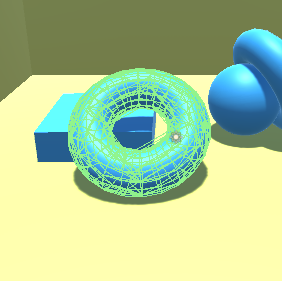
\includegraphics[scale=0.55]{images/bwp1.png}
	\end{center}
  	\caption{改良前}
  	\label{fig:bwp1}
\end{figure}

\begin{figure}[!hbt]
  	\begin{center}
  		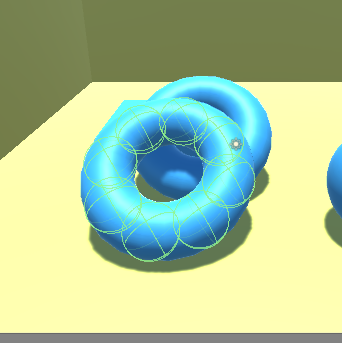
\includegraphics[scale=0.5]{images/bwp2.png}
	\end{center}
  	\caption{改良後}
  	\label{fig:bwp2}
\end{figure}

このように,円環体の当たり判定が簡略されながらも充分に実現されていることが分かる.Sphere Colliderで実現したことにより,プレハブ化してもRigidbodyとの併用が問題なく行うことができた.

\subsubsection{プランニングを行えるようにスクリプトを作成する.}
Clicked.csについて,クリックされたときにまずフォーカス対象のオブジェクトをnullにしている.次にクリックしたオブジェクトの取得をRaycastを用いて行うが,ここで操作対象外である床等のオブジェクトをフォーカス対象外にする必要があった.これはフォーカス対象のブロックにPlanというタグを統一して付けることで,CompareTagからその判定を行えるようにした.また,クリック時に円環体の当たり判定である子オブジェクトを検出したとき,親オブジェクトを取り扱うように,rootフィールドを用いてその値を取得した.

クリックしたときに実行されるUpdateメソッドは以下のとおりである.

\begin{lstlisting}[caption=ClickedクラスのUpdateメソッド, label=clicked]
    void Update()
    {
        if (Input.GetMouseButtonDown(0))
        {
            if(clickedGameObject != null)
            {
                clickedGameObject = null;
            }

            Ray ray = Camera.main.ScreenPointToRay(Input.mousePosition);
            RaycastHit hit = new RaycastHit();

            if (Physics.Raycast(ray, out hit))
            {
                clickedGameObject = hit.collider.gameObject.transform.root.gameObject;  // 親要素の取得
                if (!clickedGameObject.CompareTag("Plan"))
                {
                    clickedGameObject = null;  // Planeは対象外
                }
            }

            Debug.Log(hit.collider.gameObject);
        }
    }
\end{lstlisting}

Operating.csでは,Clickedクラスで取得したオブジェクトの移動のために,GetKeyメソッドを用いてキーボードの入力判定を行う.初めはスクリプト内で一時的に対象のオブジェクトのRigidbodyのisKinematicをtrueにしてtransformのpositionにVector3を足し合わせることで移動させていたが,それだと摩擦の判定が行われなかったり,衝突判定を貫通して移動できてしまったりするという問題があった.これはisKinematicをtrueにしたことが原因であると分かった.そこで,positionに足し合わせるのではなくAddForceでVector3を足し合わせるようにしたことで,isKinematicをfalseのまま物理的制約に準ずる物体の移動を実現することが出来た.

キーボード入力時に挙動を示すOperatingクラスは以下の様になっている.

\begin{lstlisting}[caption=Operatingクラス, label=operating]
public class Operating : MonoBehaviour
{
    private Vector3 velocity;
    private float moveSpeed = 1000.0f;

    void Update()
    {
        velocity = Vector3.zero;
        if (Input.GetKey(KeyCode.W))
            velocity.z += 1;
        if (Input.GetKey(KeyCode.A))
            velocity.x -= 1;
        if (Input.GetKey(KeyCode.S))
            velocity.z -= 1;
        if (Input.GetKey(KeyCode.D))
            velocity.x += 1;
        if (Input.GetKey(KeyCode.E))
            velocity.y += 1;
        if (Input.GetKey(KeyCode.Q))
            velocity.y -= 1;
        // 速度ベクトルの長さを1秒でmoveSpeedだけ進むように調整します
        velocity = velocity.normalized * moveSpeed * Time.deltaTime;

        if (velocity.magnitude > 0)
        {
            // プレイヤーの位置(transform.position)の更新
            // 移動方向ベクトル(velocity)を足し込みます
            GameObject go = Clicked.clickedGameObject;
            if (go != null)
            {
                go.GetComponent<Rigidbody>().AddForce(velocity);
            }
        }
    }
}
\end{lstlisting}

Generator.csでは,ResourcesクラスのLoadメソッドからプレハブを取得し,Instantiateで生成するようにすることで,任意のタイミングで好きなだけブロックの生成ができるようにした. \\

Destroyer.csでは,Clicked.cs同様にタグを用いて判定することで,ブロック以外のオブジェクトが誤って消えることのないようにした. \\

また,これらのスクリプトは各オブジェクトにアタッチせずとも,Masterオブジェクトにさえアタッチすれば全体の挙動が管理できるような仕様としたことで,各オブジェクトに対する負荷を減らし,効率的なプログラムを実装することができた.

\clearpage

\subsection{実行例}
Block World Planning.exeを起動したところ,下図のような画面が得られる.

\begin{figure}[!hbt]
  	\begin{center}
  		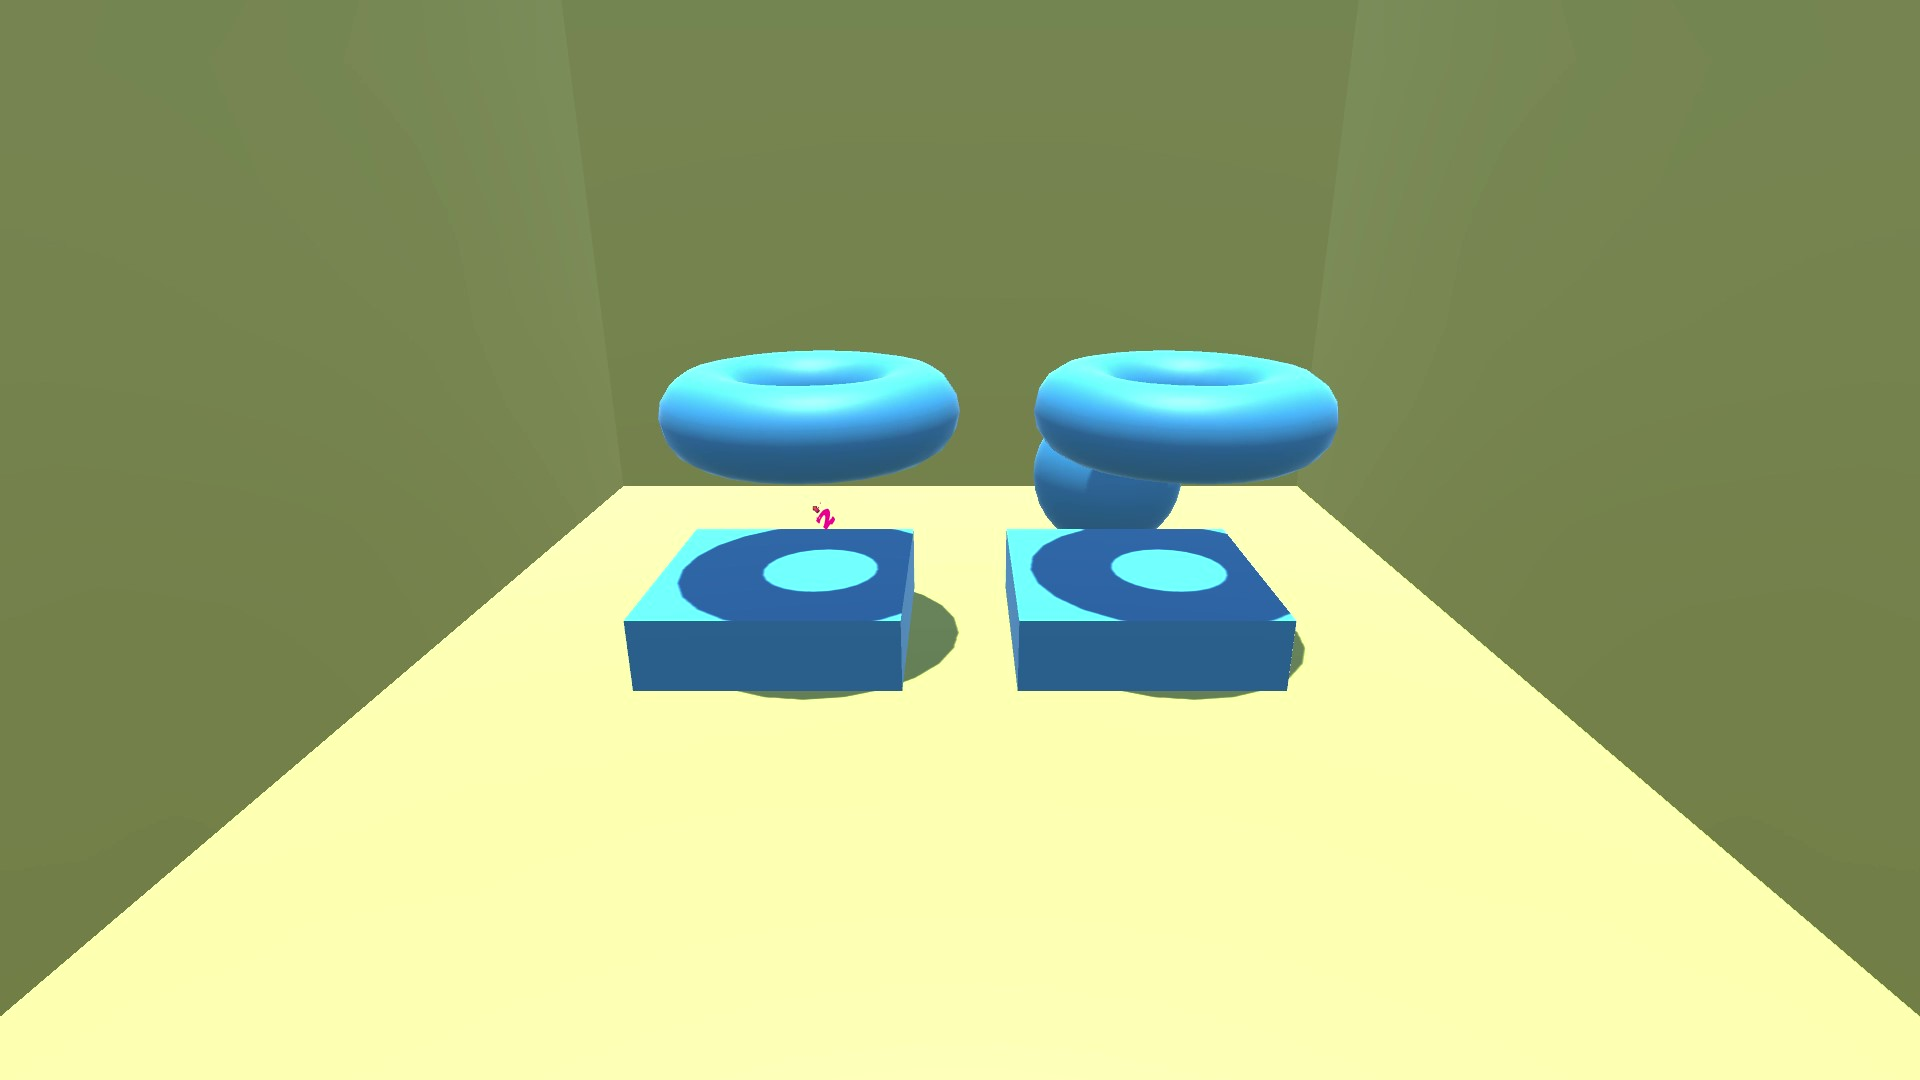
\includegraphics[scale=0.2]{images/bwp3.jpg}
	\end{center}
  	\caption{起動時の画面}
\end{figure}
\clearpage

右クリックでオブジェクトを削除でき,キー``1''で直方体,キー``2''で円環体,キー``3''で球のブロックを生成できる.これによって構成した下図をプランニングの初期状態とする.

\begin{figure}[!hbt]
  	\begin{center}
  		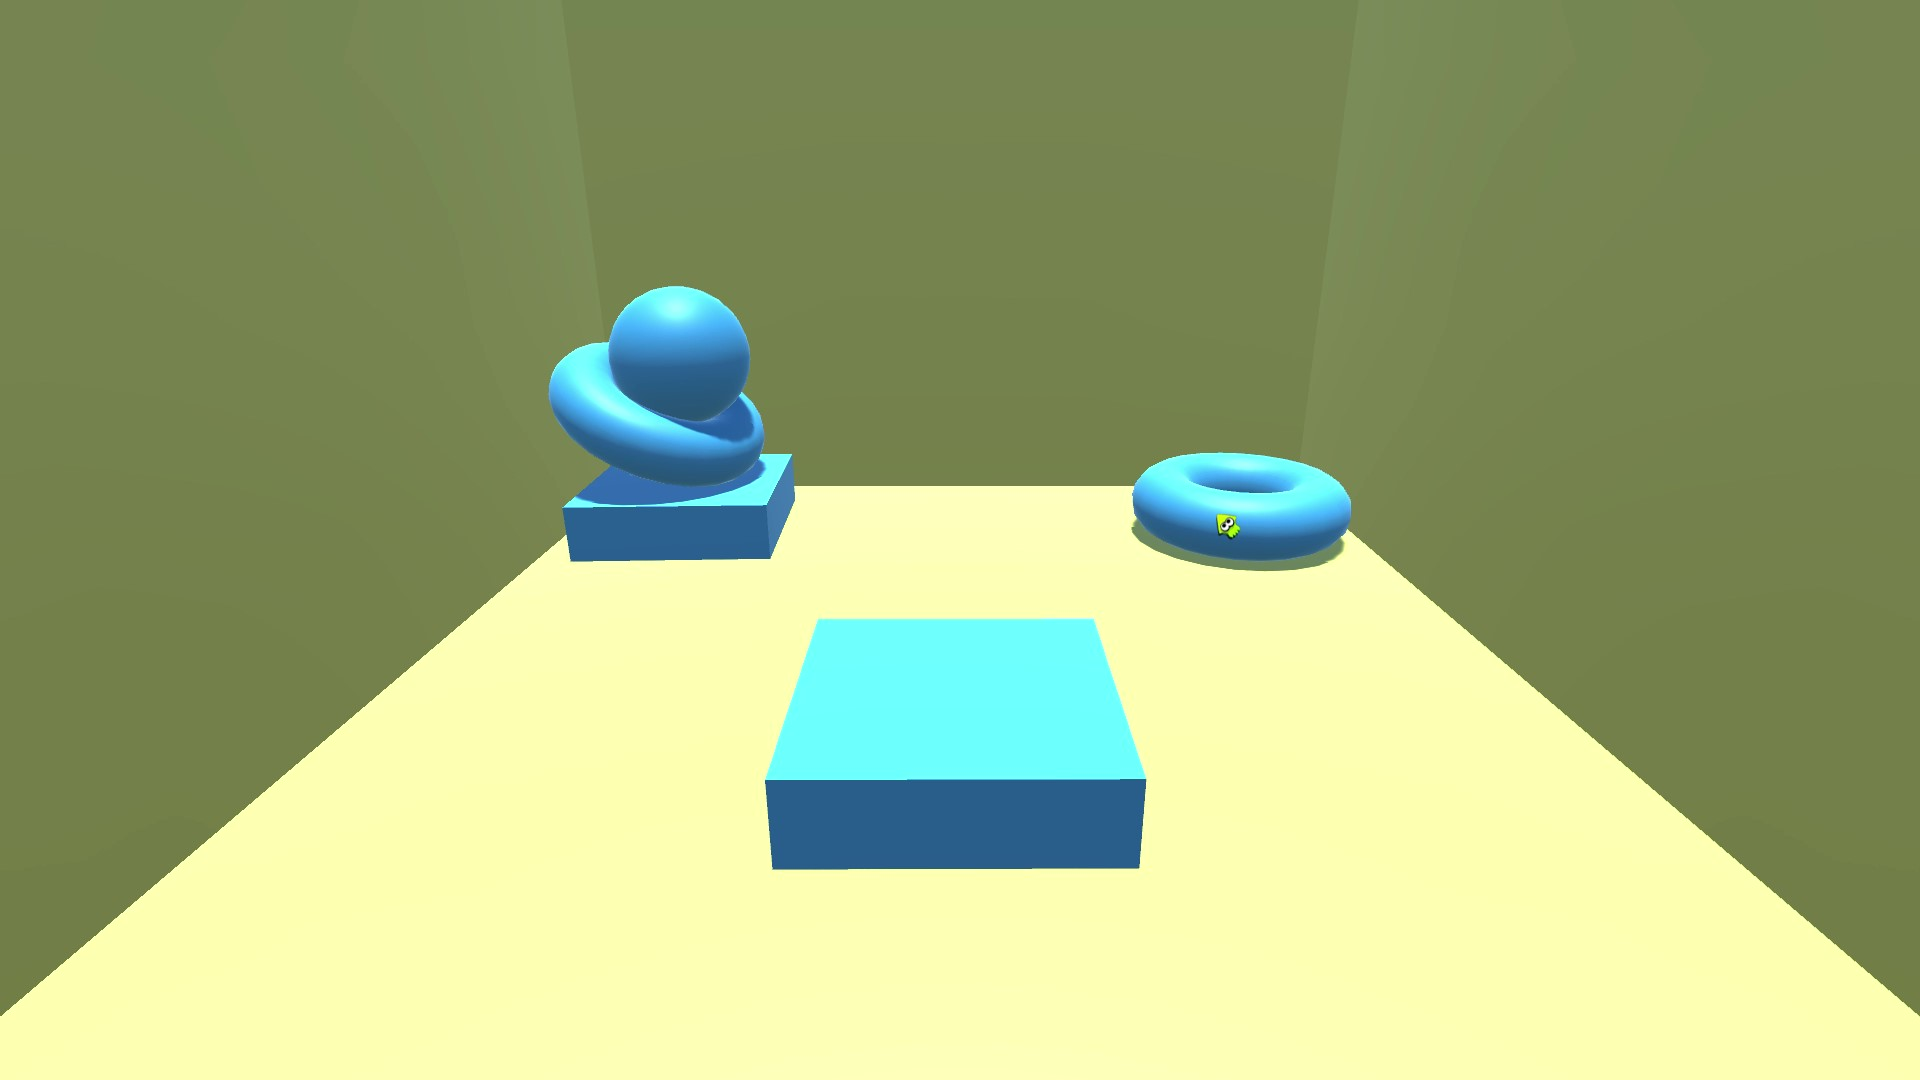
\includegraphics[scale=0.2]{images/bwp4.jpg}
	\end{center}
  	\caption{初期状態}
\end{figure}
\clearpage

左クリックで移動するオブジェクトを選択してから,WASDキーで上下左右,EQキーで昇降の移動が行える.手前の直方体に乗せるために右奥の円環体を持ち上げた様子が下図のとおりである.

\begin{figure}[!hbt]
  	\begin{center}
  		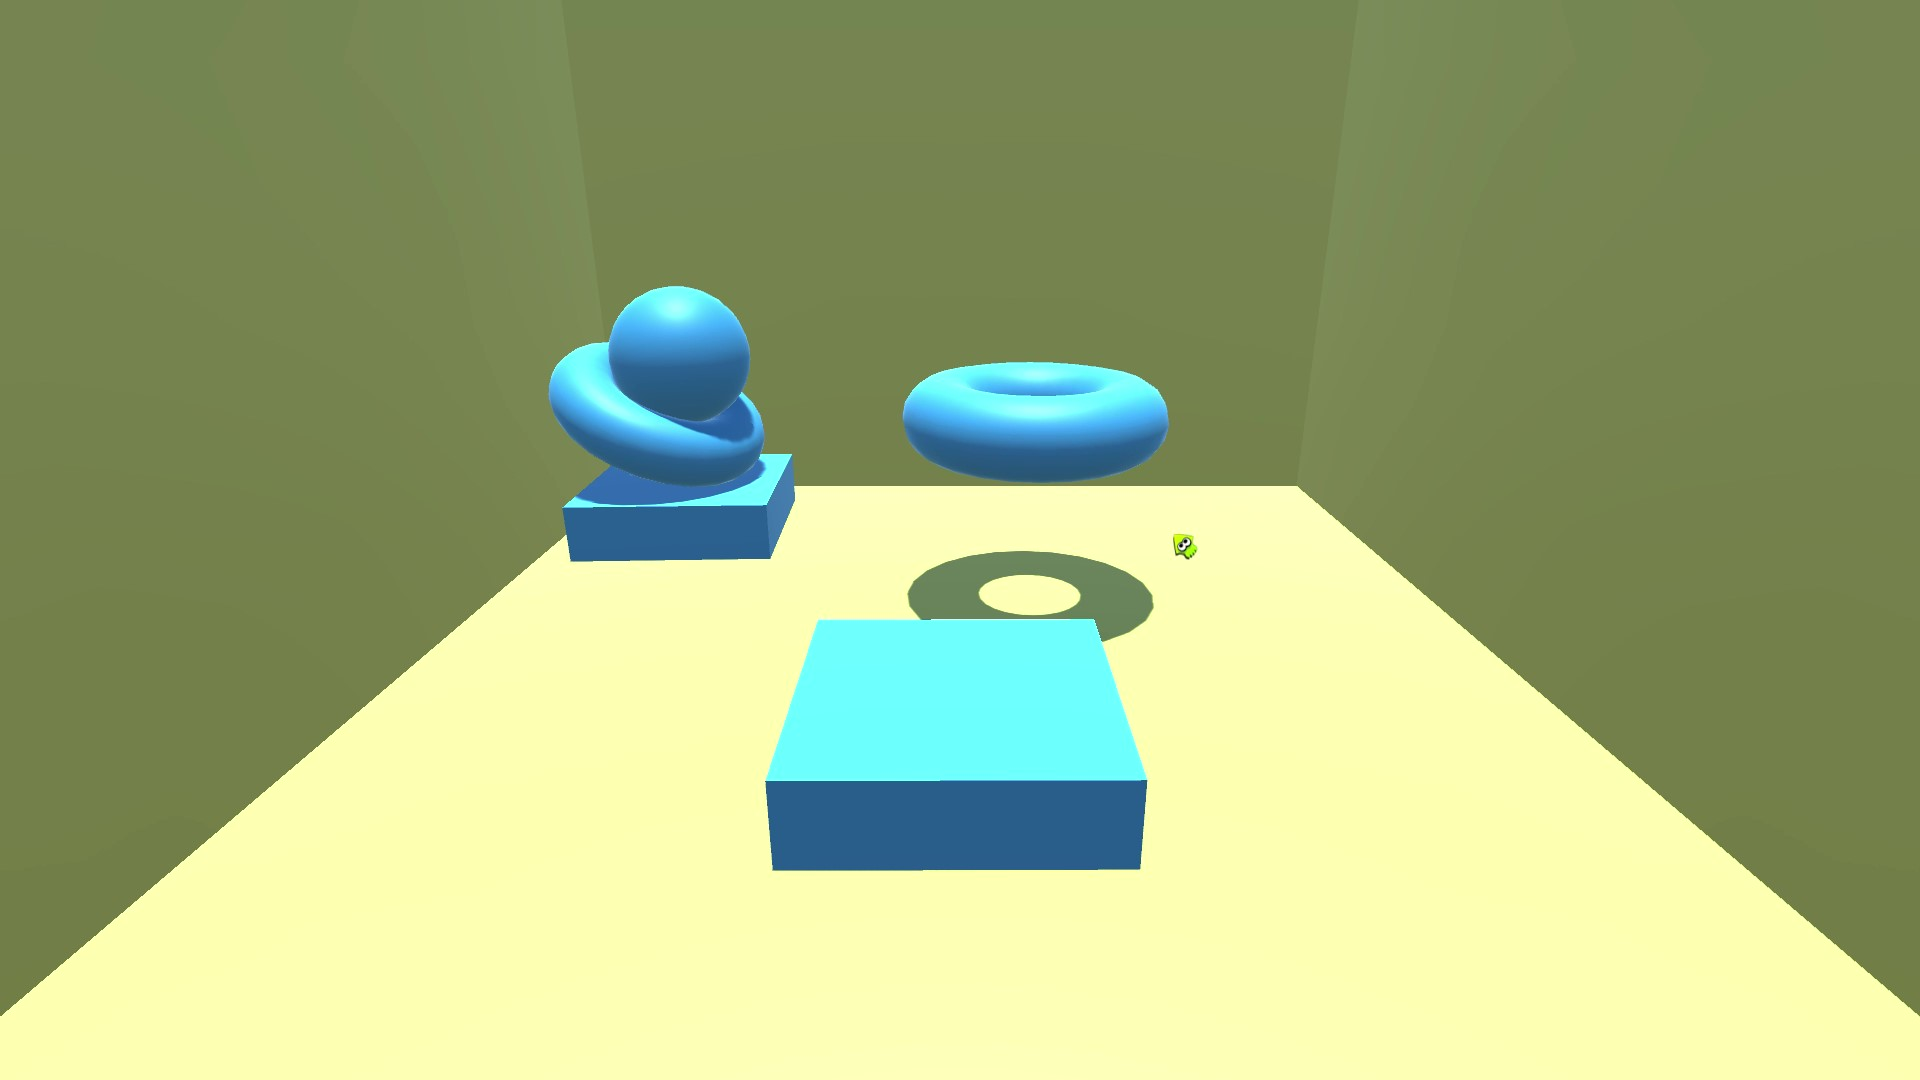
\includegraphics[scale=0.2]{images/bwp5.jpg}
	\end{center}
  	\caption{プランニング開始}
\end{figure}
\clearpage

そうして,物理的な挙動を考慮した上で円環体を直方体の上に乗せた様子が下図のとおりである.

\begin{figure}[!hbt]
  	\begin{center}
  		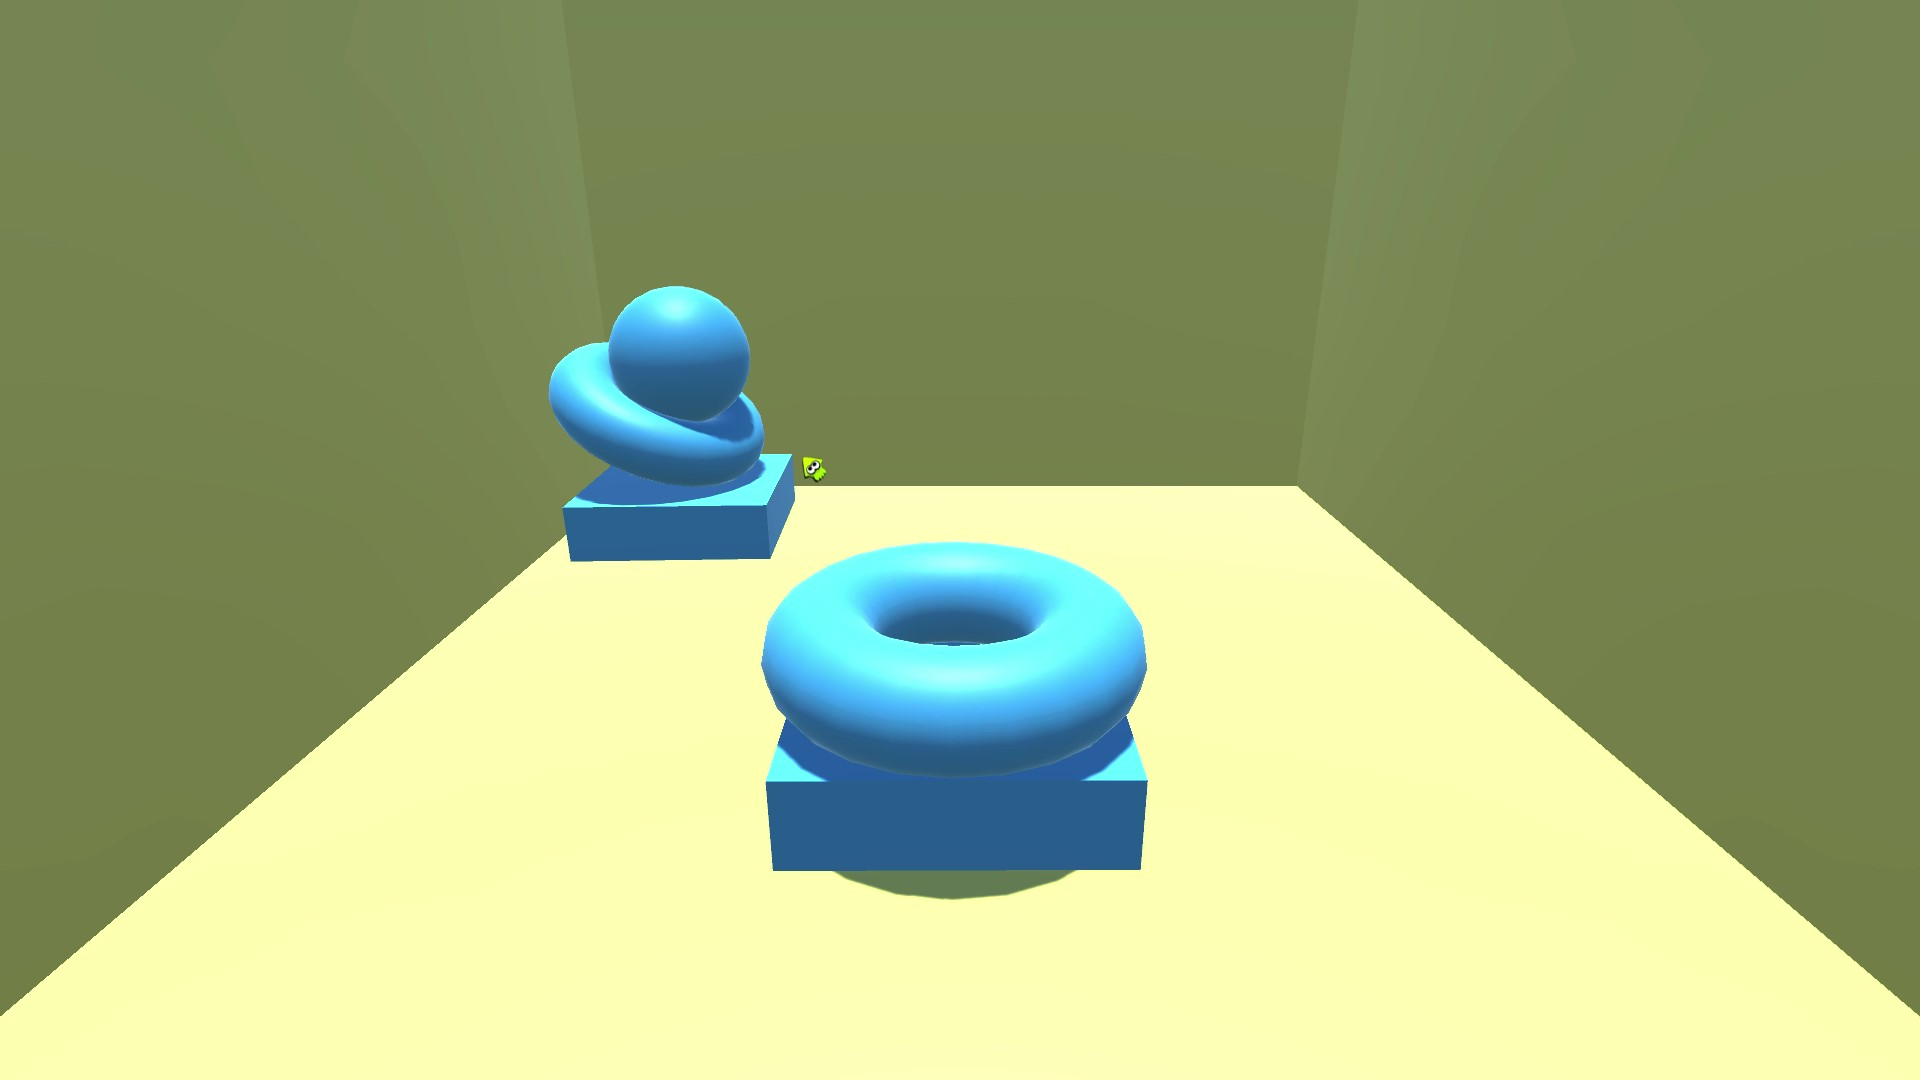
\includegraphics[scale=0.2]{images/bwp6.jpg}
	\end{center}
  	\caption{ステップ1完了}
\end{figure}
\clearpage

物理的な挙動を考慮して完了したプランニングが下図のとおりである.

\begin{figure}[!hbt]
  	\begin{center}
  		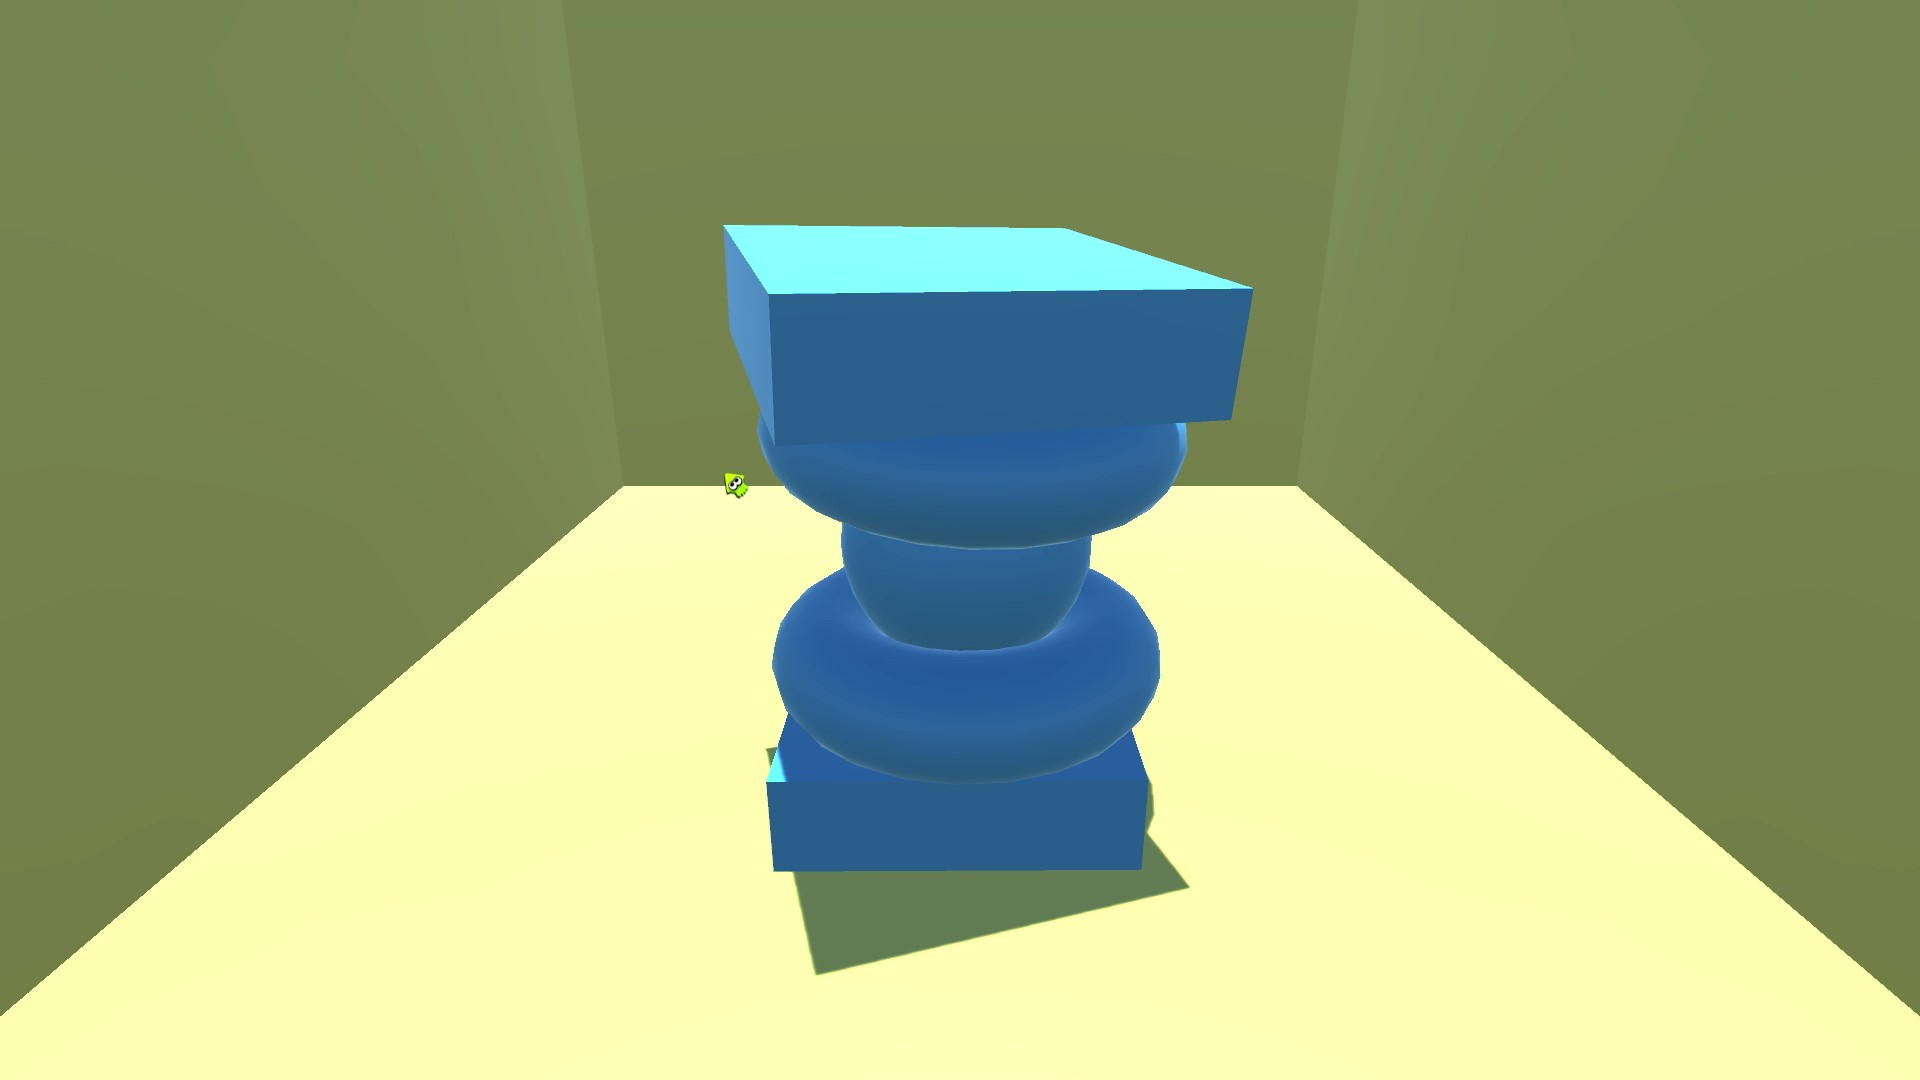
\includegraphics[scale=0.2]{images/bwp7.jpg}
	\end{center}
  	\caption{プランニング完了}
\end{figure}
\clearpage

\subsection{考察}
物理的な挙動を考慮したプランニングを実装するためにUnityを用いてみて,衝突判定や重力の考慮などを付けるだけなら容易に出来たが,円環体の穴の当たり判定が正しく設定できないなどで数多く躓いた.この問題はSphereColliderを工夫して用いることで解決したが,このように,実現したいものをマイナーなアセットを探して実現するのではなく,今ある機能を工夫して用いて実現する,という考え方は大切にすべきだと思った.

厳密な当たり判定が必要であったわけではなく,円環体の穴に自然な感じで球をはめたいというのが元々の目的であったことに気づいたおかげで解決できたように,本当に実現したいものは何か,本当に必要なものは何かを立ち返って考え,問題を簡略化することが,プログラミングの1つのテクニックであると考えられる. \\

また,子オブジェクトという概念に悩まされたように,UnityもJavaと同じ様に,ポインタが何を指しているかを考え,微妙な違いを見落とさないようにすることが重要であることを痛感した.UnityはJavaよりも並列的な処理がしやすい一方で,カプセル化に関しては大雑把な印象を受けたため,パブリックな変数がどのように遷移しているのか,Debug.Logをこまめに用いて確認することが大切だと思った. \\

また,Unityを使っていてフリーズやクラッシュが起こって,データが飛んだことがあった.Javaのプログラミングではそういうことが起こったことはなかったので,ゲームエンジンならではの重い処理の影響だと考えられる.このような普段と違うフレームワークを用いるときは,そのフレームワークに合わせてこまめにセーブをするといった対応や環境構築を行うことも大切だと考えられた. \\

また,作ったアプリをチームメンバにやってみてもらったところ,処理が重いという報告を受けた.このことを受け,フレームルートやポリゴンの制限を行い,自分とは違う環境でも動作しやすいアプリケーション作りを今後は意識してゆく必要があると思った.



\section{発展課題5-8}
\begin{screen}
    教科書3.3節のプランニング手法を応用できそうなブロック操作以外のタスクをグループで話し合い,新たなプランニング課題を自由に設定せよ.
    さらに,もし可能であれば,その自己設定課題を解くプランニングシステムを実装せよ.
\end{screen}
本課題では実装までは至らなかったので,プランニング課題のアイデア及び考察のみを記述することとする.
​
\subsection{考察}
今回のプランニングシステムを用いた課題として,システム開発のスケジュール自動生成を提案する.システム開発には多数のセクションが存在し,また多数の作業が並行して行われるのでスケジュール表は時間軸と作業分類の二次元的になる.加えて,作業の中には特定の作業が終了してからでないと取りかかれないものもある.\\
これを今回のプランニング課題に当てはめると,各作業はブロックに,作業順の制約は物理的制約に対応すると考えられ,それらの条件の元適切なスケジュール表を生成する課題は今回のプランニング課題を応用できると考える.


% 参考文献
\begin{thebibliography}{99}
\bibitem{notty} Javaによる知能プログラミング入門 --著:新谷 虎松 \\
\bibitem{Swing} Let'sプログラミング Swingを使ってみよう, \url{https://www.javadrive.jp/tutorial/} (2019年12月8日アクセス).
\end{thebibliography}

\end{document}